\documentclass{article}%
\usepackage[T1]{fontenc}%
\usepackage[utf8]{inputenc}%
\usepackage{lmodern}%
\usepackage{textcomp}%
\usepackage{lastpage}%
%
\usepackage{amsmath}%
\usepackage{amssymb}%
\usepackage{amsfonts}%
\usepackage{graphicx}%
\usepackage{hyperref}%
\usepackage{tikz}%
\usepackage{pgfplots}%
\usetikzlibrary{math}%
\title{IME 2027 - Química\thanks{This exam was solved and automatically generated with gpt-resolve: \url{https://github.com/lgabs/gpt-resolve}}}%
\author{claude{-}sonnet{-}5{-}5 (solver) + claude{-}sonnet{-}5{-}5 (judge)}%
\date{November 09, 2026}%
%
\begin{document}%
\normalsize%
\maketitle%
\section*{Questão 1}

\section*{Solução}

\textbf{Ideia.} O MnO$_2$ (pirolusita) oxida o HCl concentrado, produzindo Cl$_2$. O Cl$_2$ é mais oxidante que o Br$_2$ e por isso desloca o bromo do brometo. Assim, a massa de MnO$_2$ se obtém por estequiometria em duas etapas encadeadas.

\textbf{1) Reações envolvidas (balanceadas).}

Produção do cloro (a quente, HCl concentrado):
\[
\mathrm{MnO_2 + 4\,HCl \longrightarrow MnCl_2 + Cl_2 + 2\,H_2O}
\]
Aqui o Mn passa de $+4$ para $+2$ (reduz, $\Delta = 2$) e 2 dos 4 Cl$^-$ passam de $-1$ para $0$ (oxidam, $\Delta = 2$ no total). Os outros 2 Cl$^-$ permanecem como íons em MnCl$_2$. Portanto a equação está balanceada em átomos e em carga.

Liberação do bromo (reação de deslocamento, pois Cl$_2$ é mais oxidante que Br$_2$):
\[
\mathrm{Cl_2 + 2\,NaBr \longrightarrow 2\,NaCl + Br_2}
\]

\textbf{2) Quantidade de NaBr.} Com as massas atômicas da prova:
\[
M_{\mathrm{NaBr}} = 22{,}990 + 79{,}904 \simeq 102{,}9\ \mathrm{g\cdot mol^{-1}}
\]
\[
n_{\mathrm{NaBr}} = \frac{2{,}06\ \mathrm{g}}{102{,}9\ \mathrm{g\cdot mol^{-1}}} \simeq 2{,}00\times 10^{-2}\ \mathrm{mol}
\]

\textbf{3) Cloro necessário.} Pela segunda reação, 1 mol de Cl$_2$ libera o bromo de 2 mol de NaBr. Para liberar \emph{todo} o bromo, basta a quantidade estequiométrica de Cl$_2$:
\[
n_{\mathrm{Cl_2}} = \frac{n_{\mathrm{NaBr}}}{2} \simeq 1{,}00\times 10^{-2}\ \mathrm{mol}
\]

\textbf{4) MnO$_2$ necessário.} Pela primeira reação, 1 mol de MnO$_2$ gera 1 mol de Cl$_2$, logo
\[
n_{\mathrm{MnO_2}} = n_{\mathrm{Cl_2}} \simeq 1{,}00\times 10^{-2}\ \mathrm{mol}
\]
Somando as duas etapas (o Cl$_2$ se cancela), a reação global é
\[
\mathrm{MnO_2 + 4\,HCl + 2\,NaBr \longrightarrow MnCl_2 + 2\,NaCl + Br_2 + 2\,H_2O},
\]
com proporção $1\ \mathrm{MnO_2} : 2\ \mathrm{NaBr}$, o que confirma o resultado acima. O HCl é fornecido em excesso, pois é concentrado.

\textbf{5) Massa de MnO$_2$.}
\[
M_{\mathrm{MnO_2}} = 54{,}938 + 2\cdot 15{,}999 \simeq 86{,}94\ \mathrm{g\cdot mol^{-1}}
\]
\[
m_{\mathrm{MnO_2}} = n\,M = 1{,}00\times10^{-2}\ \mathrm{mol}\times 86{,}94\ \mathrm{g\cdot mol^{-1}} \simeq 0{,}87\ \mathrm{g}
\]

\textbf{Conferência.} A razão entre as massas é $m_{\mathrm{MnO_2}}/m_{\mathrm{NaBr}} = \dfrac{86{,}94}{2\cdot 102{,}9}\simeq 0{,}42$. De fato, $0{,}42\times 2{,}06 \simeq 0{,}87$ g. A unidade é grama e a ordem de grandeza é coerente com os poucos centimoles envolvidos. O resultado supõe rendimento de 100\% e HCl em excesso.

\textbf{Resposta:} a massa de MnO$_2$ necessária é de aproximadamente $0{,}87$ g.

ANSWER: $m_{\mathrm{MnO_2}} \simeq 0{,}87\ \mathrm{g}$ (reações: $\mathrm{MnO_2 + 4HCl \to MnCl_2 + Cl_2 + 2H_2O}$ e $\mathrm{Cl_2 + 2NaBr \to 2NaCl + Br_2}$)%
\newpage%
\section*{Questão 2}

\section*{Solução}

\textbf{Convenções e hipóteses.} Gás ideal, $n=1$ mol, sistema fechado. $W$ é o trabalho realizado \emph{sobre} o gás e a primeira lei é $\Delta U=Q+W$. Para um gás ideal $U=U(T)$ (só depende da temperatura), logo $\Delta U=\int C_V\,dT$ vale para qualquer processo, reversível ou não, e $\Delta U=0$ numa isoterma. Os estados são percorridos na ordem $1\to2\to3\to4\to1$.

\textbf{Temperaturas dos estados.} A etapa I é isotérmica: $T_2=T_1$. A etapa III começa no estado 3 e é isotérmica: $T_4=T_3$. Na etapa II (compressão adiabática, $V_3<V_2$) tem-se $Q_2=0$ e $\Delta U_2=W_2>0$ (o gás é comprimido), logo $T_3>T_1$. Na etapa IV (expansão adiabática, $V_1>V_4$) tem-se $\Delta U_4=W_4<0$ e a temperatura cai de $T_3$ para $T_1$.

\medskip\noindent\textbf{a) Gráfico $P\times V$.}

Numa isoterma, $PV=RT$ (hipérbole); a isoterma de $T_3$ fica acima da de $T_1$.

\begin{itemize}
\item \textbf{I} (lenta, $T_1$): percorre a isoterma $T_1$ de $1\,(V_1,P_1)$ até $2\,(V_2<V_1,\;P_2=P_1V_1/V_2>P_1)$.
\item \textbf{II} (rápida, adiabática): de $2$ até $3\,(V_3<V_2,\;P_3>P_2)$, passando para a isoterma de $T_3>T_1$ (sobe de forma muito inclinada).
\item \textbf{III} (lenta, $T_3$): percorre a isoterma $T_3$ de $3$ até $4\,(V_4>V_3,\;P_4<P_3)$.
\item \textbf{IV} (rápida, adiabática): de $4$ até $1$, com $V_1>V_4$ e $P_1<P_4$ (pois $P_4V_4=RT_3>RT_1=P_1V_1$ e $V_4<V_1$).
\end{itemize}

As etapas II e IV são rápidas (irreversíveis): os estados intermediários não são de equilíbrio e não existe curva $P(V)$ bem definida; por isso são traçadas \emph{tracejadas}, apenas ligando os estados extremos (e não são adiabáticas reversíveis $PV^{\gamma}=\text{const}$).

\begin{center}
\begin{tikzpicture}[x=8cm,y=1.2cm,>=stealth,font=\small]
  % eixos
  \draw[->] (0,0) -- (1.2,0) node[right] {$V$};
  \draw[->] (0,0) -- (0,6.3) node[above] {$P$};
  % isotermas de fundo (T1 e T3)
  \draw[gray!60,thin,domain=0.4:1.13,samples=50,smooth] plot (\x,{1/\x});
  \draw[gray!60,thin,domain=0.26:1.13,samples=60,smooth] plot (\x,{1.5/\x});
  \node[gray!60!black,above right] at (1.13,1.33) {$T_3$};
  \node[gray!60!black,below right] at (1.13,0.88) {$T_1$};
  % etapa I (isoterma T1) e etapa III (isoterma T3)
  \draw[very thick,domain=1:0.4,samples=40,smooth] plot (\x,{1/\x});
  \draw[very thick,domain=0.26:0.48,samples=40,smooth] plot (\x,{1.5/\x});
  % etapas II e IV (tracejadas, forma apenas ilustrativa)
  \draw[very thick,dashed,domain=0.4:0.26,samples=20,smooth] plot (\x,{2.5*exp(-1.94*ln(\x/0.4))});
  \draw[very thick,dashed,domain=0.48:1,samples=30,smooth] plot (\x,{3.125*exp(-1.552*ln(\x/0.48))});
  % setas de sentido (no meio de cada etapa)
  \draw[very thick,->] (0.66,1.515) -- (0.64,1.5625);
  \draw[very thick,->] (0.345,4.348) -- (0.355,4.225);
  \draw[very thick,->] (0.317,3.95) -- (0.309,4.12);
  \draw[very thick,->] (0.74,1.595) -- (0.76,1.531);
  % projeções nos eixos
  \draw[dotted] (1,0) -- (1,1) -- (0,1);
  \draw[dotted] (0.4,0) -- (0.4,2.5) -- (0,2.5);
  \draw[dotted] (0.26,0) -- (0.26,5.77) -- (0,5.77);
  \draw[dotted] (0.48,0) -- (0.48,3.125) -- (0,3.125);
  % estados
  \fill (1,1) circle (1.6pt) node[above right] {$1$};
  \fill (0.4,2.5) circle (1.6pt) node[below left] {$2$};
  \fill (0.26,5.77) circle (1.6pt) node[above right] {$3$};
  \fill (0.48,3.125) circle (1.6pt) node[above right] {$4$};
  % rótulos das etapas
  \node[below left] at (0.70,1.40) {\textbf{I}};
  \node[left] at (0.305,3.5) {\textbf{II}};
  \node[above right] at (0.39,4.0) {\textbf{III}};
  \node at (0.84,1.55) {\textbf{IV}};
  % marcas nos eixos
  \node[below] at (1,0) {$V_1$};
  \node[below] at (0.48,0) {$V_4$};
  \node[below] at (0.4,0) {$V_2$};
  \node[below] at (0.26,0) {$V_3$};
  \node[left] at (0,1) {$P_1$};
  \node[left] at (0,2.5) {$P_2$};
  \node[left] at (0,3.125) {$P_4$};
  \node[left] at (0,5.77) {$P_3$};
\end{tikzpicture}
\end{center}
\noindent\emph{(Esboço qualitativo, fora de escala; as setas indicam o sentido do percurso.)}

\medskip\noindent\textbf{b) Trabalho total.}

\[
W_{tot}=W_1+W_2+W_3+W_4 .
\]

As etapas II e IV são adiabáticas ($Q_2=Q_4=0$) e, por serem rápidas, irreversíveis: o trabalho nelas \emph{não} é $-\int P\,dV$ do gás, nem vale $PV^{\gamma}=\text{const}$. Mas a primeira lei dispensa o conhecimento do caminho:
\[
W_2=\Delta U_2=U(T_3)-U(T_2)=U(T_3)-U(T_1)\qquad(T_2=T_1),
\]
\[
W_4=\Delta U_4=U(T_1)-U(T_4)=U(T_1)-U(T_3)\qquad(T_4=T_3).
\]
Somando, $W_2+W_4=0$ (com $C_V$ constante, $W_2=C_V(T_3-T_1)=-W_4$). Portanto
\[
\boxed{W_{tot}=W_1+W_3}
\]
O trabalho gasto na compressão rápida é exatamente devolvido na expansão rápida, pois ambas ligam as mesmas temperaturas $T_1$ e $T_3$ e $U$ é função de estado. Como o ciclo fecha, $\Delta U_{ciclo}=0$ e $Q_{tot}=-W_{tot}=Q_1+Q_3$, coerente com $Q_2=Q_4=0$.

\textbf{Forma explícita.} Nas etapas lentas (quase estáticas), $P_{ext}\approx P=RT/V$:
\[
W_1=RT_1\ln\frac{V_1}{V_2}>0,\qquad W_3=-RT_3\ln\frac{V_4}{V_3}<0,\qquad
W_{tot}=R\left[T_1\ln\frac{V_1}{V_2}-T_3\ln\frac{V_4}{V_3}\right].
\]

\textbf{Verificação numérica.} Gás monoatômico ($C_V=\tfrac32R$), $V_2=V_1/3$, etapa II contra $P_{ext}=P_3=5P_1$ e etapa IV contra $P_{ext}=P_1$. A primeira lei na etapa II, $\tfrac32R(T_3-T_1)=P_3(V_2-V_3)$ com $P_3V_3=RT_3$, dá $T_3=\tfrac{19}{15}T_1$ e $V_3=\tfrac{19}{75}V_1$; na etapa IV, $\tfrac32R(T_1-T_3)=-P_1(V_1-V_4)$ dá $V_4=0{,}6\,V_1$. Em unidades de $RT_1=P_1V_1$: $W_2=P_3(V_2-V_3)=+0{,}40$ e $W_4=-P_1(V_1-V_4)=-0{,}40$, de fato iguais a $\Delta U=\tfrac32R\,(\pm\tfrac{4}{15}T_1)=\pm0{,}40\,RT_1$. Logo $W_2+W_4=0$, como previsto.

\medskip
ANSWER: a) ciclo formado por duas isotermas (etapa I a $T_1$ e etapa III a $T_3>T_1$) ligadas por dois trechos rápidos tracejados (II e IV); b) $W_2=\Delta U_2=U(T_3)-U(T_1)$ e $W_4=\Delta U_4=U(T_1)-U(T_3)$, logo $W_2+W_4=0$ e $W_{tot}=W_1+W_3$.%
\newpage%
\section*{Questão 3}

\section*{Solução}

\textbf{Hipótese.} Admite-se uma lei de velocidade do tipo $v = k\,[\mathrm{SO_2}]^{x}\,[\mathrm{O_3}]^{y}$. As ordens $x$ e $y$ são determinadas experimentalmente (não vêm dos coeficientes estequiométricos). Como o vaso tem volume constante, as concentrações são bem definidas. O $\mathrm{N_2}$ é inerte e não altera as concentrações dos reagentes. As velocidades da tabela são iniciais, e a temperatura é a mesma (300 K) nos três experimentos, portanto $k$ é o mesmo.

\subsection*{a) Ordens de reação}

\textbf{Ordem em $\mathrm{O_3}$ (experimentos 1 e 2).} $[\mathrm{SO_2}]$ é fixa em $0{,}25$ mol/L e $[\mathrm{O_3}]$ cai à metade, de $0{,}40$ para $0{,}20$ mol/L. A velocidade não muda:
\[
\frac{v_1}{v_2}=\left(\frac{0{,}40}{0{,}20}\right)^{y}=\frac{0{,}118}{0{,}118}=1
\;\Rightarrow\; 2^{y}=1 \;\Rightarrow\; y=0 .
\]

\textbf{Ordem em $\mathrm{SO_2}$ (experimentos 2 e 3).} $[\mathrm{O_3}]$ é fixa em $0{,}20$ mol/L e $[\mathrm{SO_2}]$ triplica, de $0{,}25$ para $0{,}75$ mol/L:
\[
\frac{v_3}{v_2}=\left(\frac{0{,}75}{0{,}25}\right)^{x}=\frac{1{,}062}{0{,}118}=9
\;\Rightarrow\; 3^{x}=9 \;\Rightarrow\; x=2 .
\]

Portanto, a reação é de \textbf{ordem 2 em $\mathrm{SO_2}$} e de \textbf{ordem 0 em $\mathrm{O_3}$}. A ordem global é 2.

\subsection*{b) Lei da velocidade}

\[
\boxed{v = k\,[\mathrm{SO_2}]^{2}}
\]

\subsection*{c) Constante de velocidade a 300 K}

Usa-se o experimento 2 (o 1 e o 3 dão o mesmo valor):
\[
k_1=\frac{v}{[\mathrm{SO_2}]^2}=\frac{0{,}118}{(0{,}25)^2}=\frac{0{,}118}{0{,}0625}\approx 1{,}89\ \text{L}\cdot\text{mol}^{-1}\cdot\text{s}^{-1}.
\]
\emph{Conferência (experimento 3):} $1{,}062/(0{,}75)^2 = 1{,}062/0{,}5625 \approx 1{,}89$. Os valores coincidem.

\emph{Unidades:} $\text{mol·L}^{-1}\text{·s}^{-1} = k\,(\text{mol·L}^{-1})^{2}$ implica $k$ em $\text{L·mol}^{-1}\text{·s}^{-1}$, como esperado para ordem global 2.

\subsection*{d) Energia de ativação}

Pela equação de Arrhenius, $k = A\,e^{-E_a/RT}$. Escrevendo-a para duas temperaturas e dividindo uma pela outra, $A$ se cancela:
\[
\ln\frac{k_2}{k_1}=\frac{E_a}{R}\left(\frac{1}{T_1}-\frac{1}{T_2}\right)
\;\Rightarrow\;
E_a=\frac{R\,\ln(k_2/k_1)}{\dfrac{1}{T_1}-\dfrac{1}{T_2}} .
\]

Dados: $T_1=300$ K, $k_1\approx1{,}89$, $T_2=1000$ K, $k_2=7{,}56$ (mesma unidade de $k_1$, pois a lei de velocidade é a mesma).

Razão das constantes:
\[
\frac{k_2}{k_1}=\frac{7{,}56}{1{,}89}=4{,}00
\;\Rightarrow\;
\ln 4 = 2\ln 2 \simeq 1{,}386 .
\]

Diferença de inversos das temperaturas:
\[
\frac{1}{300}-\frac{1}{1000}=\frac{10-3}{3000}=\frac{7}{3000}\ \text{K}^{-1}.
\]

Substituindo, com $R=8{,}3$ J·mol$^{-1}$·K$^{-1}$:
\[
E_a=\frac{8{,}3\times 1{,}386}{7/3000}=8{,}3\times1{,}386\times\frac{3000}{7}\approx 4{,}93\times10^{3}\ \text{J/mol}.
\]

\[
\boxed{E_a \approx 4{,}9\ \text{kJ}\cdot\text{mol}^{-1}}
\]

\emph{Conferência.}
\begin{itemize}
\item O resultado é positivo, como deve ser, e $k$ aumenta com $T$.
\item Usando $k_1=1{,}888$ sem arredondar, $k_2/k_1=4{,}004$ e $E_a\approx 4{,}93$ kJ/mol, praticamente o mesmo valor.
\item Uma $E_a$ baixa é compatível com a reação ser iniciada por radiação UV e com o pequeno ganho de $k$ (cerca de 4 vezes) para um aumento de $700$ K.
\end{itemize}

\medskip
\noindent ANSWER: a) ordem 2 em $\mathrm{SO_2}$ e ordem 0 em $\mathrm{O_3}$ (global 2); b) $v=k[\mathrm{SO_2}]^2$; c) $k\approx1{,}89\ \text{L·mol}^{-1}\text{·s}^{-1}$; d) $E_a\approx4{,}9\ \text{kJ/mol}$ ($\approx 4{,}93\times10^{3}$ J/mol).%
\newpage%
\section*{Questão 4}

\section*{Solução}

\textbf{Modelo e leitura do dado.} A auto-associação é $2\,\mathrm{CH_3COOH}\rightleftharpoons(\mathrm{CH_3COOH})_2$ (monômero $M$, dímero $D$), com $K_c=\dfrac{[D]}{[M]^2}$. Leio ``cada mol de monômero (dissolvido) gera $0{,}42$ mol de dímero'' de forma literal: $n_D=0{,}42\,n_0$, sendo $n_0$ o ácido total dissolvido (o máximo possível seria $0{,}5\,n_0$). Cada dímero consome 2 monômeros, logo, para $1{,}00$ mol de ácido dissolvido,
\[
n_D=0{,}42\ \text{mol},\qquad n_M=1-2(0{,}42)=0{,}16\ \text{mol},\qquad \alpha=0{,}84 .
\]
A relação dímero/monômero do equilíbrio é, portanto, $n_D/n_M=0{,}42/0{,}16=2{,}625$.

\textbf{a)} A interação é a \emph{ligação (ponte) de hidrogênio}: o H da hidroxila (H ligado a O, muito eletronegativo) de uma molécula atrai um par isolado do O carbonílico ($\mathrm{C{=}O}$) da outra, formando $\mathrm{O{-}H\cdots O{=}C}$. São duas pontes por dímero, que fecham um anel de 8 átomos (por isso ``cíclico''). O dímero é praticamente apolar (os dipolos das duas metades se cancelam), o que explica a boa solubilidade em benzeno, solvente apolar que não compete pelas pontes e favorece a dimerização.

\textbf{b)} Cada monômero $\mathrm{C_2H_4O_2}$ tem $2(4)+4(1)+2(6)=24$ elétrons de valência; o dímero tem $48$. Em cada monômero há $8$ pares ligantes ($3$ C--H, C--C, C=O (2), C--O, O--H) e $4$ pares isolados (2 em cada O). As pontes de hidrogênio \emph{não} são ligações covalentes (não há par compartilhado entre os monômeros): são interações eletrostáticas, desenhadas em pontilhado. Desenho esquemático (a geometria real do anel não é retangular):
\begin{center}
\begin{tikzpicture}[scale=1.35, every node/.style={font=\small}]
  \node (CL) at (0,0) {C};
  \node (CR) at (4.4,0) {C};
  \node (MeL) at (-1.5,0) {H$_3$C};
  \node (MeR) at (5.9,0) {CH$_3$};
  \node (OLt) at (0.9,1.3) {O};
  \node (OLb) at (0.9,-1.3) {O};
  \node (ORt) at (3.5,1.3) {O};
  \node (ORb) at (3.5,-1.3) {O};
  \node (Ht) at (2.55,1.3) {H};
  \node (Hb) at (1.85,-1.3) {H};
  \draw (MeL) -- (CL);
  \draw (CR) -- (MeR);
  \draw[double, double distance=1.4pt] (CL) -- (OLt);
  \draw (CL) -- (OLb);
  \draw (CR) -- (ORt);
  \draw[double, double distance=1.4pt] (CR) -- (ORb);
  \draw (Ht) -- (ORt);
  \draw (OLb) -- (Hb);
  \draw[dotted, thick] (OLt) -- (Ht);
  \draw[dotted, thick] (Hb) -- (ORb);
  \foreach \n/\a in {OLt/70, OLt/140, OLb/200, OLb/280, ORt/10, ORt/100, ORb/340, ORb/260}{
    \fill ([shift={(\a+11:0.27)}]\n.center) circle (0.03);
    \fill ([shift={(\a-11:0.27)}]\n.center) circle (0.03);
  }
  \node[font=\footnotesize] at (2.2,2.0) {ligações de hidrogênio (pontilhado)};
\end{tikzpicture}
\end{center}

\textbf{c)} $K_c$ exige concentrações, e a única concentração fornecida é $0{,}10\ \text{mol}\cdot\text{L}^{-1}$, no item (d). O enunciado diz que essa solução \emph{preserva a relação dímero/monômero} do equilíbrio. Como $K_c$ é constante (mesma $T$), $R=[D]/[M]=K_c\,[M]$; manter $R$ equivale a manter $[M]$ e, pela estequiometria, também $[D]$ e a concentração total. Logo a solução de (d) \emph{é} o próprio estado de equilíbrio, e $c_0=0{,}10$ mol$\cdot$L$^{-1}$. (Em geral, $K_c=\dfrac{0{,}42}{0{,}16^{2}\,c_0}=\dfrac{16{,}4}{c_0}$: um $c_0$ diferente daria outro $K_c$, mas contrariaria a hipótese de (d).) Então
\[
[M]=0{,}16\,c_0=0{,}016\ \text{mol/L},\qquad [D]=0{,}42\,c_0=0{,}042\ \text{mol/L},
\]
\[
K_c=\frac{[D]}{[M]^2}=\frac{0{,}042}{(0{,}016)^2}=\frac{0{,}042}{2{,}56\times10^{-4}}\approx 1{,}6\times 10^{2}\ \text{L}\cdot\text{mol}^{-1}\quad(\approx 164).
\]
Verificação: $[M]+2[D]=0{,}016+0{,}084=0{,}100$ mol/L, conservando o ácido. A ordem de grandeza ($10^2$ L/mol) é a esperada para a dimerização forte do ácido acético em solvente apolar.

\textbf{d)} Solvente benzeno: $T_f^{\,0}=5{,}45\ ^\circ\mathrm{C}$, $K_f=5{,}12\ \mathrm{K\cdot kg\cdot mol^{-1}}$. Hipóteses: solução diluída e ideal, soluto não volátil e que não cristaliza com o solvente, volumes aditivos. Então $\Delta T=K_f\,W$, com $W$ a molalidade \emph{de partículas} (monômeros livres mais dímeros; cada dímero conta como uma partícula):
\[
[M]+[D]=0{,}016+0{,}042=0{,}058\ \text{mol/L}\qquad(i=1-\alpha/2=0{,}58).
\]
Massa de solvente em 1 L de solução: o ácido ($M_r=60{,}05$) ocupa $\dfrac{0{,}10\cdot 60{,}05}{1{,}05\cdot 10^{3}}\approx 5{,}7\times10^{-3}$ L, restando $0{,}994$ L de benzeno, isto é, $m=0{,}87\cdot0{,}994\approx0{,}865$ kg. Assim
\[
W=\frac{0{,}058}{0{,}865}\approx 0{,}0671\ \text{mol/kg},\qquad
\Delta T=5{,}12\cdot 0{,}0671\approx 0{,}34\ \text{K},
\]
\[
T_f=5{,}45-0{,}34\approx 5{,}11\ ^\circ\mathrm{C}.
\]
(Aproximando $1$ L de solução $\approx 0{,}87$ kg de benzeno obtém-se $W=0{,}0667$ e $T_f=5{,}109\ ^\circ$C, o mesmo valor com 3 algarismos.) Conferência: sem associação ($i=1$) seria $\Delta T\approx0{,}59$ K; a dimerização reduz o número de partículas e, por isso, o abaixamento ($0{,}34<0{,}59$ K), e $\Delta T\ll T_f^{\,0}$ confirma a validade da lei.

\textbf{Observação (leitura alternativa).} Se ``$0{,}42$'' fosse lido como a razão $[D]/[M]=0{,}42$ no equilíbrio, com $[M]+2[D]=0{,}10$ mol/L se obteria $[M]\approx0{,}054$, $[D]\approx0{,}023$ mol/L, $K_c\approx7{,}7$ L/mol e $T_f\approx5{,}00\ ^\circ$C. Descarto essa leitura porque o enunciado fala em ``\emph{cada mol} de monômero \emph{gera} $0{,}42$ mol de dímero'' (produto por mol de ácido dissolvido, como adotado) e porque $K_c\approx 8$ L/mol subestimaria a associação do ácido acético em benzeno, que é fortíssima ($\sim10^2$ L/mol).

\medskip
\noindent ANSWER: a) ligações (pontes) de hidrogênio $\mathrm{O{-}H\cdots O{=}C}$; b) dímero cíclico de 8 átomos com duas pontes de hidrogênio (figura); c) $K_c\approx 1{,}6\times10^{2}\ \text{L/mol}$ (164 L/mol, para $c_0=0{,}10$ mol/L); d) $T_f\approx 5{,}11\ ^\circ\mathrm{C}$.%
\newpage%
\section*{Questão 5}

\section*{Solução}

\textbf{Ideia.} Os dois calorímetros medem grandezas diferentes: a volume constante, $\Delta U$; a pressão constante, $\Delta H$. A diferença entre as elevações de temperatura depende só de $\Delta H-\Delta U$, isto é, da variação do número de mols gasosos, $\Delta n$. Calcula-se $\Delta n$ a partir dos dados e compara-se com o de cada candidato.

\textbf{Hipóteses.} (i) Gases ideais. (ii) Todo o calor da reação é absorvido pelo calorímetro, de capacidade térmica constante $C=450\ \text{J}\cdot\text{K}^{-1}$ (conteúdo incluído). (iii) Os dois experimentos partem do mesmo estado inicial, a $27\ ^\circ\text{C}=300\ \text{K}$, e $\Delta U$ e $\Delta H$ são referidos a essa temperatura, como diz o item (i) do enunciado. (iv) Combustão completa com todas as espécies gasosas, logo $\text{H}_2\text{O}$ em forma de vapor.

\textbf{1) Calor absorvido em cada calorímetro (1,0 mol queimado).}
\begin{itemize}
\item Volume constante: não há trabalho de expansão, então $q_V=\Delta U$ e $C\,\Delta T_V=-\Delta U$.
\item Pressão constante: $q_P=\Delta H$ e $C\,\Delta T_P=-\Delta H$.
\end{itemize}
A combustão é exotérmica, então $\Delta T_V>0$ e $\Delta T_P>0$.

\textbf{2) Relação entre $\Delta H$ e $\Delta U$.}
Para gases ideais, $pV=nRT$. Com $T$ igual nos dois casos,
\[
\Delta H=\Delta U+\Delta(pV)=\Delta U+\Delta n\,RT,
\]
em que $\Delta n=n_{\text{gás,produtos}}-n_{\text{gás,reagentes}}$ (por mol de substância queimada, contando o combustível e o $\text{O}_2$ como reagentes). Subtraindo as duas relações do passo 1:
\[
C\,(\Delta T_V-\Delta T_P)=\Delta H-\Delta U=\Delta n\,RT .
\]
Como $\Delta T_V-\Delta T_P=16{,}6>0$, resulta $\Delta n>0$.

\textbf{3) Valor de $\Delta n$.}
Um intervalo de $16{,}6\ ^\circ\text{C}$ equivale a $16{,}6\ \text{K}$. Logo
\[
\Delta n=\frac{C\,(\Delta T_V-\Delta T_P)}{RT}=\frac{450\cdot 16{,}6}{8{,}3\cdot 300}=\frac{7470}{2490}=3{,}0 .
\]
Unidades: $\text{J}\cdot\text{K}^{-1}\cdot\text{K}\,/\,(\text{J}\cdot\text{mol}^{-1}\cdot\text{K}^{-1}\cdot\text{K})=\text{mol}$.

\textbf{4) $\Delta n$ de cada candidato.}
Todos são hidrocarbonetos $\text{C}_x\text{H}_y$:
\[
\text{C}_x\text{H}_y(g)+\left(x+\tfrac{y}{4}\right)\text{O}_2(g)\longrightarrow x\,\text{CO}_2(g)+\tfrac{y}{2}\,\text{H}_2\text{O}(g),
\]
\[
\Delta n=x+\tfrac{y}{2}-1-\left(x+\tfrac{y}{4}\right)=\frac{y}{4}-1 .
\]
Portanto $\Delta n=3$ exige $y=16$. A última coluna da tabela mostra o valor de $\Delta T_V-\Delta T_P=\Delta n\,RT/C$ que cada composto produziria:

\begin{center}
\begin{tabular}{lcccc}
Composto & Fórmula & $y$ & $\Delta n=y/4-1$ & $\Delta T_V-\Delta T_P$ \\ \hline
acetileno & $\text{C}_2\text{H}_2$ & 2 & $-0{,}5$ & $-2{,}8\ \text{K}$ \\
p-xileno & $\text{C}_8\text{H}_{10}$ & 10 & $+1{,}5$ & $+8{,}3\ \text{K}$ \\
n-heptano & $\text{C}_7\text{H}_{16}$ & 16 & $+3{,}0$ & $+16{,}6\ \text{K}$ \\
propeno & $\text{C}_3\text{H}_6$ & 6 & $+0{,}5$ & $+2{,}8\ \text{K}$ \\
\end{tabular}
\end{center}

\textbf{5) Verificação e exclusões.}
Para o n-heptano, $\text{C}_7\text{H}_{16}+11\,\text{O}_2\to 7\,\text{CO}_2+8\,\text{H}_2\text{O}$ dá $\Delta n=15-12=3$. Então $\Delta T_V-\Delta T_P=\dfrac{3\cdot 8{,}3\cdot 300}{450}=16{,}6\ \text{K}$, exatamente o dado.
\begin{itemize}
\item Acetileno: $\Delta n<0$ daria $\Delta T_V<\Delta T_P$, contra o enunciado.
\item Propeno ($+2{,}8$ K) e p-xileno ($+8{,}3$ K): têm sinal correto, mas o valor não bate com $16{,}6$ K.
\end{itemize}
Só o n-heptano satisfaz o valor.

\textbf{Comentário sobre ordem de grandeza.} 1 mol de heptano libera cerca de $4{,}8\cdot 10^{6}\ \text{J}$, o que, com $C=450\ \text{J}\cdot\text{K}^{-1}$, daria $\Delta T$ absolutos da ordem de $10^{4}$ K, irrealistas. A questão é idealizada: apenas a diferença $\Delta T_V-\Delta T_P$ é usada, e nela os termos de $\Delta U$ comuns se cancelam, restando só $\Delta n\,RT/C$.

\textbf{Conclusão.} A substância queimada foi o \textbf{n-heptano} ($\text{C}_7\text{H}_{16}$), o único com $\Delta n=+3$.

ANSWER: n-heptano ($\text{C}_7\text{H}_{16}$), pois $\Delta n_{\text{gás}}=C\,(\Delta T_V-\Delta T_P)/(RT)=+3$ e só ele tem $y=16$.%
\newpage%
\section*{Questão 6}

\section*{Solução}

\textbf{Dados e hipóteses.} Massas molares aproximadas: ácido acético $\mathrm{CH_3COOH}$ ($\mathrm{C_2H_4O_2}$) $\approx 60$ g/mol; etanol $\mathrm{C_2H_5OH}$ ($\mathrm{C_2H_6O}$) $\approx 46$ g/mol. Como só há equilíbrio líquido-líquido (condição i), todas as espécies, inclusive a água, estão numa única fase líquida homogênea. Admite-se solução ideal, com atividades $\approx$ concentrações, e por isso a água entra na expressão de $K_c$. As condições (ii) e (iii), volume, $T$ e $P$ constantes, fazem $K_c$ ter um único valor e $V$ ser o mesmo para todas as espécies.

\textbf{Quantidades iniciais}
\[
n_{\text{ác}}^{0}=\frac{240}{60}=4{,}0\ \text{mol},\qquad n_{\text{et}}^{0}=\frac{92}{46}=2{,}0\ \text{mol}.
\]

\textbf{a) Equação balanceada} (esterificação de Fischer, proporção 1:1:1:1):
\[
\mathrm{CH_3COOH}(l)\;+\;\mathrm{C_2H_5OH}(l)\;\rightleftharpoons\;\mathrm{CH_3COOC_2H_5}(l)\;+\;\mathrm{H_2O}(l)
\]
Os produtos são o acetato de etila e a água. Conferência dos átomos: reagentes $\mathrm{C_2H_4O_2}+\mathrm{C_2H_6O}=\mathrm{C_4H_{10}O_3}$; produtos $\mathrm{C_4H_8O_2}+\mathrm{H_2O}=\mathrm{C_4H_{10}O_3}$. Cada lado tem 4 C, 10 H e 3 O, logo a equação está balanceada.

\textbf{Tabela de equilíbrio.} Seja $x$ o número de mols de cada produto formado. O enunciado dá $x=1{,}6$ mol. Pela estequiometria 1:1:1:1, ácido e etanol são consumidos em $x$ mol cada.

\begin{center}
\begin{tabular}{l c c c c}
 & ácido & etanol & éster & água \\ \hline
início (mol) & 4,0 & 2,0 & 0 & 0 \\
variação (mol) & $-1{,}6$ & $-1{,}6$ & $+1{,}6$ & $+1{,}6$ \\
equilíbrio (mol) & 2,4 & 0,4 & 1,6 & 1,6 \\
\end{tabular}
\end{center}

O etanol é o reagente limitante ($2{,}0<4{,}0$). Como $1{,}6<2{,}0$, todas as quantidades no equilíbrio são positivas, e a reação é incompleta, como deve ser num equilíbrio.

\textbf{b) Grau de equilíbrio para o ácido acético.} É a fração do ácido inicial que reagiu até o equilíbrio:
\[
\alpha_{\text{ác}}=\frac{n_{\text{consumido}}}{n^{0}_{\text{ác}}}=\frac{1{,}6}{4{,}0}=0{,}40\quad(40\,\%).
\]
Observação: o grau pedido refere-se ao ácido, e não ao etanol. Em relação ao etanol, que é o limitante, a conversão seria $1{,}6/2{,}0=80\,\%$.

\textbf{c) Constante de equilíbrio.} Seja $V$ o volume da mistura, constante e comum a todas as espécies, de modo que $[i]=n_i/V$. Então
\[
K_c=\frac{[\text{éster}]\,[\text{H}_2\text{O}]}{[\text{ácido}]\,[\text{etanol}]}
=\frac{\dfrac{1{,}6}{V}\cdot\dfrac{1{,}6}{V}}{\dfrac{2{,}4}{V}\cdot\dfrac{0{,}4}{V}}
=\frac{1{,}6\cdot 1{,}6}{2{,}4\cdot 0{,}4}.
\]
Como $\Delta n=0$ (2 mol de reagentes e 2 mol de produtos por mol de reação), $V$ se cancela. Por isso não é preciso conhecer o volume, e $K_c$ é adimensional:
\[
K_c=\frac{2{,}56}{0{,}96}=\frac{8}{3}\approx 2{,}67 .
\]

\textbf{Verificações independentes.}
\begin{itemize}
\item \emph{Conservação de massa:} $2{,}4\cdot 60+0{,}4\cdot 46+1{,}6\cdot 88+1{,}6\cdot 18=144+18{,}4+140{,}8+28{,}8=332$ g, igual a $240+92=332$ g. A conservação de carbono também fecha: $2(2{,}4)+2(0{,}4)+4(1{,}6)=12=2(4)+2(2)$ mol de C.
\item \emph{Consistência de $K_c$:} com $K_c=8/3$ e as quantidades iniciais dadas, $x^2/[(4-x)(2-x)]=8/3$ leva a $5x^2-48x+64=0$, cujas raízes são $x=1{,}6$ e $x=8$. A raiz $x=8$ é fisicamente impossível, pois $x\le 2{,}0$. Assim, $x=1{,}6$ é a única solução admissível.
\item \emph{Sentido da reação:} no início $Q=0<K_c$, de modo que a reação avança no sentido dos produtos, como observado.
\item \emph{Arredondamento:} com as massas molares da tabela, $60{,}05$ e $46{,}07$ g/mol, obtém-se $\alpha\approx 0{,}400$ e $K_c\approx 2{,}69$. Isso equivale a $2{,}67$ dentro da precisão dos dados (as massas molares aproximadas $60$ e $46$ dão $8/3$).
\end{itemize}

\textbf{Resultados:} a) $\mathrm{CH_3COOH(l)+C_2H_5OH(l)\rightleftharpoons CH_3COOC_2H_5(l)+H_2O(l)}$; b) $\alpha=0{,}40$ (40\,\%); c) $K_c=8/3\approx 2{,}67$.

\medskip
\noindent ANSWER: a) $\mathrm{CH_3COOH + C_2H_5OH \rightleftharpoons CH_3COOC_2H_5 + H_2O}$; b) $\alpha = 0{,}40$ (40\,\%); c) $K_c = 8/3 \approx 2{,}67$ (adimensional)%
\newpage%
\section*{Questão 7}

\section*{Solução}

\textbf{1. Por que uma lei de potências? (estado estacionário).} X é um intermediário reativo: $[\mathrm{X}]_0=0$ e ele é consumido nas etapas II e III assim que se forma. Após um período de indução muito curto, $d[\mathrm{X}]/dt\approx 0$:
\[
k_1[\mathrm{A}][\mathrm{B}]=\bigl(k_2[\mathrm{B}]+k_3[\mathrm{C}]\bigr)[\mathrm{X}]
\;\Rightarrow\;
\nu_0=k_2[\mathrm{X}][\mathrm{B}]=\frac{k_1k_2[\mathrm{A}][\mathrm{B}]^2}{k_2[\mathrm{B}]+k_3[\mathrm{C}]}.
\]
Isso só tem forma de potência simples em dois limites: (i) $k_2[\mathrm{B}]\gg k_3[\mathrm{C}]$, com $\nu_0=k_1[\mathrm{A}][\mathrm{B}]$, ou seja, $(1,1,0)$; (ii) $k_3[\mathrm{C}]\gg k_2[\mathrm{B}]$, com $\nu_0=\dfrac{k_1k_2}{k_3}\dfrac{[\mathrm{A}][\mathrm{B}]^2}{[\mathrm{C}]}$, ou seja, $(1,2,-1)$. Esse é o sentido de \emph{``em determinadas condições''}. Os expoentes, porém, serão obtidos \textbf{dos dados}, e o mecanismo servirá de confirmação.

\textbf{2. Sistema de equações (item a).} Dividindo $\nu_0=k[\mathrm{A}]^{\alpha}[\mathrm{B}]^{\beta}[\mathrm{C}]^{\gamma}$ de cada experimento pelo do experimento 1, $k$ se cancela. Todas as razões de concentração são potências de 2, então basta igualar os expoentes de 2:
\begin{align*}
\text{2/1: }& 4{,}00=2^{\alpha}4^{\beta}8^{\gamma}\ \Rightarrow\ \alpha+2\beta+3\gamma=2,\\
\text{3/1: }& 1{,}00=4^{\alpha}2^{\beta}16^{\gamma}\ \Rightarrow\ 2\alpha+\beta+4\gamma=0,\\
\text{4/1: }& \nu_4/\nu_1=8^{\alpha}16^{\beta}2^{\gamma}\ \Rightarrow\ 3\alpha+4\beta+\gamma=\log_2(\nu_4/\nu_1).
\end{align*}
\emph{Sobre o experimento 4.} A tabela impressa traz $\nu_4=1{,}28\times10^{-6}$, o que daria $\nu_4/\nu_1=1{,}024$ e $\log_2 1{,}024\approx0{,}034$. Adoto $\nu_4=1{,}28\times10^{-3}\ \mathrm{mol\,L^{-1}s^{-1}}$ (erro de expoente na impressão), porque:
\begin{itemize}
\item a mantissa $1{,}28=1{,}25\times1{,}024$ e $1{,}024\times10^{3}=2^{10}$: a razão vira exatamente $2^{10}=1024$, e uma coincidência dessas dificilmente é acaso;
\item o valor literal leva a expoentes não inteiros e com $\alpha<0$ (ver abaixo), o que é impossível aqui, pois A só entra como reagente na etapa I e só pode acelerar a formação de P.
\end{itemize}
Com $\nu_4/\nu_1=1024=2^{10}$, a terceira equação é $3\alpha+4\beta+\gamma=10$.

\textbf{3. Resolução e unicidade.} A matriz dos coeficientes tem determinante
$\begin{vmatrix}1&2&3\\2&1&4\\3&4&1\end{vmatrix}=-15+20+15=20\neq0$, portanto a solução é única. Eliminando:
\[
2\cdot(\text{2/1 da 2ª})-(\text{1ª}):\ 3\alpha+5\gamma=-2;\qquad
(\text{3ª})-4\cdot(\text{2ª}):\ -5\alpha-15\gamma=10\ \Rightarrow\ \alpha+3\gamma=-2 .
\]
Substituindo $\alpha=-2-3\gamma$ na primeira: $-6-4\gamma=-2$, logo $\gamma=-1$, $\alpha=1$ e, pela 2ª equação, $\beta=-2\alpha-4\gamma=2$. Conferência: $1+4-3=2$; $2+2-4=0$; $3+8-1=10$.
\[
\boxed{\alpha=1,\qquad\beta=2,\qquad\gamma=-1}
\]
\emph{Valor literal (para comparação).} Com $\log_2 1{,}024\approx0{,}034$ na 3ª equação, a solução é $\alpha\approx-1{,}49$, $\beta\approx1{,}00$, $\gamma\approx0{,}495$. Esses números não são inteiros, $\alpha<0$ contradiz o mecanismo, e o resultado não corresponde a nenhum dos limites da seção 1. Isso reforça a hipótese de erro de impressão.

\textbf{4. Confirmação independente pelo mecanismo.} Seja $r=k_3/k_2$. A lei completa da seção 1 dá, para as razões com o experimento 1,
\[
\frac{\nu_2}{\nu_1}=\frac{8(1+r)}{1+2r},\qquad
\frac{\nu_3}{\nu_1}=\frac{8(1+r)}{1+8r},\qquad
\frac{\nu_4}{\nu_1}=\frac{1024(1+r)}{8+r}.
\]
Com $r=0$ (limite i) obtém-se $8,\,8,\,128$, incompatível com os dados. Já para $r\gg1$ (limite ii) obtém-se $4,\,1,\,1024$. Os experimentos 2 e 3, que não dependem do erro de impressão, já exigem esse limite, e com ele a família de soluções de (2/1, 3/1) fica restrita a $(1,2,-1)$. Portanto o experimento 4 corrigido e o mecanismo chegam, por caminhos distintos, ao mesmo resultado. Fisicamente, C compete por X na etapa III (inativa) e inibe a formação de P, o que explica $\gamma<0$ (o expoente não é coeficiente estequiométrico).

\textbf{5. Constante cinética (item b).} Pelo experimento 1, que não depende do erro de impressão:
\[
k=\frac{\nu_0[\mathrm{C}]}{[\mathrm{A}][\mathrm{B}]^2}
=\frac{1{,}25\times10^{-6}\cdot1{,}0\times10^{-2}}{1{,}0\times10^{-2}\cdot(1{,}0\times10^{-2})^2}
=1{,}25\times10^{-2}.
\]
Unidades: $\dfrac{(\mathrm{mol\,L^{-1}s^{-1}})(\mathrm{mol\,L^{-1}})}{(\mathrm{mol\,L^{-1}})^{3}}=\mathrm{L\,mol^{-1}\,s^{-1}}$. Logo
\[
\boxed{k=1{,}25\times10^{-2}\ \mathrm{L\,mol^{-1}\,s^{-1}}}\qquad(k=k_1k_2/k_3).
\]
Verificação: $[\mathrm{A}][\mathrm{B}]^2/[\mathrm{C}]=4{,}0\times10^{-4}$ (exp. 2), $1{,}0\times10^{-4}$ (exp. 3) e $1{,}024\times10^{-1}$ (exp. 4). Isso dá $\nu_0=5{,}00\times10^{-6}$, $1{,}25\times10^{-6}$ e $1{,}28\times10^{-3}$, respectivamente. Os dois primeiros coincidem com a tabela, e o terceiro coincide com o valor corrigido.

\textbf{6. Lei cinética (item c).}
\[
\boxed{\nu_0=1{,}25\times10^{-2}\,\frac{[\mathrm{A}][\mathrm{B}]^{2}}{[\mathrm{C}]}}
\quad(\text{concentrações em }\mathrm{mol\,L^{-1}},\ \nu_0\text{ em }\mathrm{mol\,L^{-1}s^{-1}}).
\]

\textbf{7. Ordem global (item d).}
\[
n=\alpha+\beta+\gamma=1+2-1=2\quad(\text{segunda ordem}),
\]
compatível com a unidade de $k$, $\mathrm{L\,mol^{-1}s^{-1}}$.

ANSWER: $\alpha=1,\ \beta=2,\ \gamma=-1$; $k=1{,}25\times10^{-2}\ \mathrm{L\,mol^{-1}\,s^{-1}}$; $\nu_0=1{,}25\times10^{-2}\,[\mathrm{A}][\mathrm{B}]^2/[\mathrm{C}]$; ordem global $=2$.%
\newpage%
\section*{Questão 8}

\section*{Solução}

\textbf{1. Reação (Wurtz).} Cloreto de alquila e sódio metálico em meio anidro acoplam dois grupos alquila:
\[
2\,\mathrm{R{-}Cl} + 2\,\mathrm{Na} \longrightarrow \mathrm{R{-}R} + 2\,\mathrm{NaCl}.
\]
Assim, $2$ mol de X e $2$ mol de Na (``quantidade equivalente'') dão $1$ mol de Y $=\mathrm{R{-}R}$, um alcano \emph{simétrico} com $2n$ carbonos, se X tem $n$ carbonos.

\textbf{2. Natureza de Y.} Um composto com dois carbonos quirais que não desvia a luz polarizada é uma forma \emph{meso}. Os dois estereocentros têm configurações opostas e se compensam internamente (plano de simetria ou centro de inversão), de modo que a molécula é sobreponível à sua imagem especular. Esses centros são trocados pela simetria da molécula, logo cada metade R contém um estereocentro.

\textbf{3. Menor Y possível.} Um carbono quiral precisa de quatro grupos diferentes. O menor R que o contém é o \emph{sec}-butila, $\mathrm{{-}CH(CH_3)CH_2CH_3}$, com $\mathrm{H}$, $\mathrm{CH_3}$, $\mathrm{C_2H_5}$ e a ligação ao outro R.
\begin{itemize}
\item $n=3$ ($\mathrm{Y}$ com $6$ C): R $=$ propila ou isopropila dá hexano ou 2,3-dimetilbutano, sem carbono quiral.
\item $n=4$ ($\mathrm{Y}$ com $8$ C): n-butila, isobutila e terc-butila dão octano, 2,5-dimetilhexano e 2,2,3,3-tetrametilbutano, sem carbono quiral. Só a \emph{sec}-butila dá $\mathrm{CH_3CH_2CH(CH_3){-}CH(CH_3)CH_2CH_3}$, com C3 e C4 quirais.
\end{itemize}
Logo, Y é o \textbf{3,4-dimetil-hexano} ($\mathrm{C_8H_{18}}$) na forma \textbf{meso}, $(3R,4S)\equiv(3S,4R)$. Os isômeros $(3R,4R)$ e $(3S,4S)$ são enantiômeros ativos e não servem.

\textbf{a) Estrutura tridimensional de Y.} Cunha cheia indica ligação para o observador e traço tracejado indica ligação para trás. À esquerda está a cadeia em zigue-zague (conformação anti, com centro de inversão entre C3 e C4). À direita está a projeção de Fischer (conformação eclipsada, com plano de simetria horizontal entre C3 e C4, e os dois $\mathrm{CH_3}$ do mesmo lado).
\[
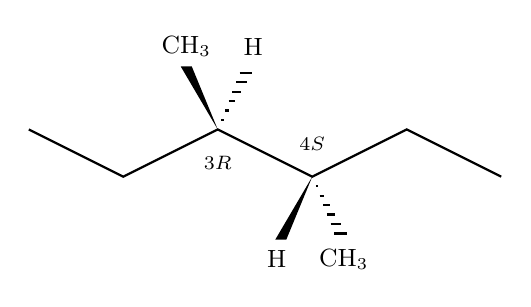
\begin{tikzpicture}[font=\small]
  \draw[thick] (-1.2,0.6)--(0,0)--(1.2,0.6)--(2.4,0)--(3.6,0.6)--(4.8,0);
  % C3: CH3 em cunha, H tracejado
  \fill (1.2,0.6) -- (0.73,1.4) -- (0.87,1.4) -- cycle;
  \foreach \t in {0.15,0.3,0.45,0.6,0.75,0.9}{\draw[line width=0.8pt] ({1.2+0.4*\t-0.09*\t},{0.6+0.8*\t}) -- ({1.2+0.4*\t+0.09*\t},{0.6+0.8*\t});}
  \node at (0.8,1.65) {$\mathrm{CH_3}$};
  \node at (1.65,1.65) {$\mathrm{H}$};
  % C4: CH3 tracejado, H em cunha
  \fill (2.4,0) -- (1.93,-0.8) -- (2.07,-0.8) -- cycle;
  \foreach \t in {0.15,0.3,0.45,0.6,0.75,0.9}{\draw[line width=0.8pt] ({2.4+0.4*\t-0.09*\t},{-0.8*\t}) -- ({2.4+0.4*\t+0.09*\t},{-0.8*\t});}
  \node at (2.8,-1.05) {$\mathrm{CH_3}$};
  \node at (1.95,-1.05) {$\mathrm{H}$};
  \node at (1.2,0.18) {\scriptsize $3R$};
  \node at (2.4,0.42) {\scriptsize $4S$};
\end{tikzpicture}
\qquad\qquad
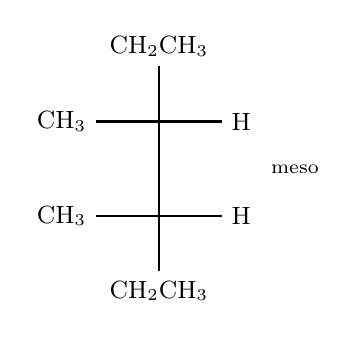
\begin{tikzpicture}[font=\small]
  \draw[thick] (0,-1.3)--(0,1.3);
  \draw[thick] (-0.8,0.6)--(0.8,0.6);
  \draw[thick] (-0.8,-0.6)--(0.8,-0.6);
  \node at (0,1.55) {$\mathrm{CH_2CH_3}$};
  \node at (0,-1.55) {$\mathrm{CH_2CH_3}$};
  \node[left] at (-0.8,0.6) {$\mathrm{CH_3}$};
  \node[right] at (0.8,0.6) {$\mathrm{H}$};
  \node[left] at (-0.8,-0.6) {$\mathrm{CH_3}$};
  \node[right] at (0.8,-0.6) {$\mathrm{H}$};
  \node[right] at (1.3,0) {\scriptsize meso};
\end{tikzpicture}
\]
\emph{Conferência CIP} (em C3: $\mathrm{C4}(\mathrm{C,C,H})>\mathrm{C2}(\mathrm{C,H,H})>\mathrm{CH_3}>\mathrm{H}$, e analogamente em C4). No zigue-zague, C3 com $\mathrm{CH_3}$ em cunha e $\mathrm{H}$ tracejado (afastado do observador) é $R$. C4, com $\mathrm{CH_3}$ tracejado e $\mathrm{H}$ em cunha, é $S$. Em Fischer, os dois $\mathrm{CH_3}$ à esquerda também dão $(3R,4S)$. Configurações opostas e grupos idênticos nos dois centros confirmam a forma meso.

\textbf{b) Nomenclatura de X.} Como $\mathrm{R}=\mathrm{{-}CH(CH_3)CH_2CH_3}$, tem-se $\mathrm{X}=\mathrm{CH_3CH_2CHClCH_3}$. A cadeia principal tem $4$ C (butano) e o Cl fica no carbono $2$ (menor localizador):
\[
\boxed{\text{X} = \text{2-clorobutano}}
\]
A equação global é
\[
2\,\mathrm{CH_3CH_2CHClCH_3} + 2\,\mathrm{Na} \to \mathrm{CH_3CH_2CH(CH_3)CH(CH_3)CH_2CH_3} + 2\,\mathrm{NaCl}.
\]
O 2-clorobutano é quiral. Para formar a meso, X deve fornecer um grupo $R$ e um $S$ (X racêmico, por exemplo). A reação não é estereosseletiva e gera meso $+$ $(3R,4R)$ $+$ $(3S,4S)$. Y é o diastereoisômero meso.

\textbf{Verificação.} $2\times4=8$ C e $\mathrm{C_8H_{18}}$ ($2n+2=18$, alcano saturado). Com $n=3$ não há Y quiral, então $8$ C é o mínimo.

ANSWER: a) Y = 3,4-dimetil-hexano na forma meso (3R,4S), desenhado acima. b) X = 2-clorobutano.%
\newpage%
\section*{Questão 9}

\section*{Solução}

\textbf{1) Massa molar de A (crioscopia).}
Hipóteses: solução diluída, soluto molecular e não volátil, só o solvente congela (sem solução sólida) e A não se dissocia nem se associa no benzeno (fator de van't Hoff $i=1$). Nessas condições, $\Delta T_c = K_c\,W$:
\begin{align*}
W&=\frac{\Delta T_c}{K_c}=\frac{1{,}28}{5{,}12}=0{,}25\ \text{mol}\cdot\text{kg}^{-1},\\
n_A&=W\,m_{\text{solv}}=0{,}25\cdot 2=0{,}50\ \text{mol},\\
M_A&=\frac{53\ \text{g}}{0{,}50\ \text{mol}}=106\ \text{g}\cdot\text{mol}^{-1}.
\end{align*}
\emph{Validade das hipóteses.} (i) Diluição: $n_{\text{benzeno}}\simeq 2000/78\simeq 25{,}6$ mol, logo $x_A\simeq 0{,}5/26{,}1\simeq 0{,}02$. (ii) Associação ($i<1$): se A formasse dímeros, o número de partículas seria $n_A/2$, o que daria $n_A=1{,}0$ mol e $M_A=53$ g/mol, menor que a massa do próprio benzeno (78 g/mol), absurdo para um composto aromático. (iii) Dissociação ($i=2$) daria $M_A=212$ g/mol, mas o benzeno é apolar ($\varepsilon\simeq 2{,}3$) e não estabiliza íons; logo $i=1$. A temperatura de fusão e a densidade do benzeno não são necessárias, pois a massa de solvente foi dada.

\textbf{2) Fórmula molecular.}
Um composto aromático tem anel benzênico ($\mathrm{C_6}$, 72 g/mol), restando $34$ g/mol para os H do anel e os substituintes (C, H, O).
\begin{itemize}
\item Monossubstituído $\mathrm{C_6H_5\!-\!R}$ (77 g/mol): $\mathrm{R}=29$ g/mol, ou seja, $-\mathrm{C_2H_5}$ ou $-\mathrm{CHO}$. (O grupo $-\mathrm{N{=}NH}$ também pesa 29, mas o fenildiazeno é instável e foge ao escopo.)
\item Dissubstituído $\mathrm{C_6H_4R_2}$ (76 g/mol): $\mathrm{R+R'}=30$ g/mol, e só serve $2\times(-\mathrm{CH_3})$. Outros pares somam 31 ($\mathrm{NH_2}+\mathrm{CH_3}$), 32 ($\mathrm{OH}+\mathrm{CH_3}$) ou mais.
\item Tri ou mais substituído: restariam $\le 31$ g/mol para três grupos de pelo menos 15 g/mol cada, impossível.
\end{itemize}
Assim, $\mathrm{C_8H_{10}}$ ($106{,}17$ g/mol): etilbenzeno e o-, m-, p-xileno; $\mathrm{C_7H_6O}$ ($106{,}12$ g/mol): benzaldeído.

\textbf{3) Teste de Tollens negativo.}
O reagente de Tollens oxida aldeídos, inclusive aromáticos, e deposita prata metálica:
\begin{multline*}
\mathrm{C_6H_5CHO + 2\,[Ag(NH_3)_2]^+ + 3\,OH^-}\\
\mathrm{\longrightarrow C_6H_5COO^- + 2\,Ag\!\downarrow + 4\,NH_3 + 2\,H_2O}.
\end{multline*}
O resultado negativo exclui o benzaldeído. Os hidrocarbonetos $\mathrm{C_8H_{10}}$ não reagem.

\textbf{4) Halogenação com um único produto.}
O critério é o número de monoderivados halogenados \emph{possíveis} (não o majoritário). Examino as duas leituras clássicas: (a) substituição eletrofílica no anel ($\mathrm{X_2/FeX_3}$); (b) substituição radicalar na cadeia lateral ($\mathrm{X_2}$, luz).
\begin{center}
\begin{tabular}{lcc}
 & (a) anel & (b) cadeia lateral \\ \hline
etilbenzeno & 3 (o, m, p) & 2 ($\alpha$ e $\beta$) \\
o-xileno & 2 (H3$\equiv$H6; H4$\equiv$H5) & 1 \\
m-xileno & 3 (H2; H4$\equiv$H6; H5) & 1 \\
p-xileno & \textbf{1} (4 H equivalentes) & \textbf{1} \\
\end{tabular}
\end{center}
O etilbenzeno dá mais de um produto nas duas leituras. Os o- e m-xilenos só dão produto único na leitura (b). O p-xileno é o único que dá produto único nas duas, e é o único possível na leitura (a), que é a que distingue os isômeros. Cada condição de reação dá um único monoderivado para ele: 2-halo-1,4-dimetilbenzeno no anel, ou $\mathrm{CH_3\!-\!C_6H_4\!-\!CH_2X}$ na cadeia.

\textbf{5) Conclusão.}
A é o \textbf{p-xileno} (1,4-dimetilbenzeno), $\mathrm{C_8H_{10}}$:

\begin{center}
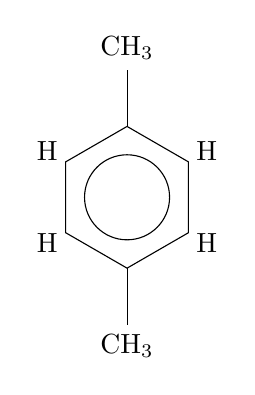
\begin{tikzpicture}[scale=0.9]
  \draw (90:1) -- (30:1) -- (-30:1) -- (-90:1) -- (-150:1) -- (150:1) -- cycle;
  \draw (0,0) circle (0.6);
  \draw (90:1) -- (90:1.8) node[above] {$\mathrm{CH_3}$};
  \draw (-90:1) -- (-90:1.8) node[below] {$\mathrm{CH_3}$};
  \node at (30:1.3) {H}; \node at (-30:1.3) {H}; \node at (150:1.3) {H}; \node at (-150:1.3) {H};
\end{tikzpicture}
\end{center}

\emph{Conferência.} $0{,}50\ \text{mol}\times 106{,}17\ \text{g/mol}\simeq 53$ g e $\Delta T_c=5{,}12\cdot 0{,}50/2=1{,}28\ ^\circ\mathrm{C}$. O produto da halogenação no anel é o 2-cloro-1,4-dimetilbenzeno (\texttt{Cc1ccc(C)c(Cl)c1}, se X = Cl).

ANSWER: A é o p-xileno (1,4-dimetilbenzeno), $\mathrm{C_8H_{10}}$, $M=106$ g/mol.%
\newpage%
\section*{Questão 10}

\section*{Solução}

\textbf{Hipóteses.} Todo o $^{208}$Pb é radiogênico (não havia Pb inicial) e o sistema permaneceu fechado desde a formação do mineral. Os intermediários da série do $^{232}$Th têm meias-vidas muito menores que $1{,}41\times10^{10}$ anos. Assim, cada átomo de $^{232}$Th que decai resulta, em escala geológica, em um átomo de $^{208}$Pb. O decaimento é de primeira ordem.

\textbf{1) Lei do decaimento.} Seja $N_0$ o número de átomos de $^{232}$Th na formação e $N_{\mathrm{Th}}$ o número atual:
\[
N_{\mathrm{Th}}=N_0\,e^{-\lambda t},\qquad \lambda=\frac{\ln 2}{t_{1/2}} .
\]
Pela conservação dos átomos, o $^{208}$Pb formado é
\[
N_{\mathrm{Pb}}=N_0-N_{\mathrm{Th}}=N_{\mathrm{Th}}\left(e^{\lambda t}-1\right).
\]

\textbf{2) Uso da razão medida.} Como $\dfrac{N_{\mathrm{Pb}}}{N_{\mathrm{Th}}}=0{,}024$ (razão molar $=$ razão atômica),
\[
e^{\lambda t}-1=0{,}024\;\Rightarrow\; e^{\lambda t}=1{,}024 \;\Rightarrow\; t=\frac{\ln(1{,}024)}{\lambda}=t_{1/2}\,\frac{\ln(1{,}024)}{\ln 2}.
\]

\textbf{3) Cálculo de $\ln 1{,}024$ com os dados fornecidos.} Note que
\[
1{,}024=\frac{1024}{1000}=\frac{2^{10}}{2^{3}\cdot 5^{3}}=\frac{2^{7}}{5^{3}}
\;\Rightarrow\;
\ln 1{,}024=7\ln 2-3\ln 5\simeq 7(0{,}693)-3(1{,}609)=4{,}851-4{,}827=0{,}024 .
\]
(Isso coincide com $\ln(1+x)\simeq x$ para $x=0{,}024$ pequeno.)

\textbf{4) Idade.} Com $t_{1/2}(^{232}\mathrm{Th})=1{,}41\times10^{10}$ anos:
\[
t=1{,}41\times10^{10}\cdot\frac{0{,}024}{0{,}693}\simeq 1{,}41\times10^{10}\cdot 0{,}0346\simeq 4{,}9\times10^{8}\ \text{anos}.
\]

\textbf{Conferência.}
\begin{itemize}
\item Ordem de grandeza: $t\ll t_{1/2}$ (aproximadamente $0{,}035\,t_{1/2}$), coerente com apenas $2{,}4\%$ do Th ter virado Pb.
\item Sem a aproximação logarítmica, $\ln(1{,}024)=0{,}02372$ dá $t\simeq 4{,}8\times10^{8}$ anos. A diferença é de cerca de $1\%$, dentro da precisão dos dados.
\item Os teores $9\%$ de $\mathrm{ThO_2}$ e $0{,}35\%$ de $\mathrm{U_3O_8}$ e a meia-vida do $^{238}$U não são necessários para a idade, pois a razão $^{208}\mathrm{Pb}/^{232}\mathrm{Th}$ já fixa $t$. O $^{238}$U só serviria se fosse dada a razão $^{206}\mathrm{Pb}/^{238}\mathrm{U}$, que forneceria uma segunda datação independente.
\end{itemize}

\textbf{Resultado:} a amostra tem idade da ordem de $4{,}9\times10^{8}$ anos (cerca de $490$ milhões de anos).

ANSWER: $t=t_{1/2}\,\dfrac{\ln(1{,}024)}{\ln 2}\simeq 4{,}9\times10^{8}$ anos%
\newpage%
\section*{Apêndice: parecer do avaliador}%
\subsection*{Questão 1: nota 9,3 (aprovada, rodada 1 de 1)}%
\textbf{Resposta da resolução às cegas do avaliador:} m(MnO$_{2}$) $\approx$ 0,87 g (0,0100 mol). Reações: MnO$_{2}$ + 4 HCl $\to$ MnCl$_{2}$ + Cl$_{2}$ + 2 H$_{2}$O e Cl$_{2}$ + 2 NaBr $\to$ 2 NaCl + Br$_{2}$. Estequiometria: 2,06 g NaBr $\approx$ 0,0200 mol $\to$ 0,0100 mol Cl$_{2}$ $\to$ 0,0100 mol MnO$_{2}$ $\to$ 0,87 g (rendimento 100 \%, HCl em excesso).\par %
Conferi o enunciado no PDF original (1ª questão, p. 2) e ele coincide com a transcrição. Refiz a conta em Python: n(NaBr) = 2,06/102,894 = 0,02002 mol, n(Cl$_{2}$) = 0,01001 mol e m(MnO$_{2}$) = 0,8703 g, o que dá $\approx$ 0,87 g. A resposta final do candidato é idêntica à da minha referência e está correta, tanto no valor quanto nas reações: MnO$_{2}$ + 4HCl $\to$ MnCl$_{2}$ + Cl$_{2}$ + 2H$_{2}$O e Cl$_{2}$ + 2NaBr $\to$ 2NaCl + Br$_{2}$. As duas reações estão balanceadas, com o Mn indo de +4 a +2 e a razão 1 Cl$_{2}$ : 2 NaBr, o que evita o erro do fator 2 (1,74 g). O candidato evita todas as armadilhas listadas: não usa MnO ou massas molares mal somadas, não mistura a quantidade de HCl com a de MnO$_{2}$, declara rendimento de 100\% e HCl em excesso, e dá a unidade correta. Ele ainda acrescenta a reação global MnO$_{2}$ + 4HCl + 2NaBr $\to$ MnCl$_{2}$ + 2NaCl + Br$_{2}$ + 2H$_{2}$O, com razão 1:2, como checagem cruzada. A resolução é clara, organizada e completa, e só tem falhas menores: a conferência final é pouco independente (e 0,42 $\times$ 2,06 = 0,865), a justificativa do deslocamento Cl$_{2}$/Br$_{2}$ é só afirmada, e as hipóteses poderiam ser mais explícitas. Está perto de um gabarito comentado publicável.%
\begin{itemize}%
\item%
{[}minor{]} A "Conferência" final é quase circular. Ela só recalcula a razão de massas 86,94/(2$\cdot$102,9) $\approx$ 0,42 e multiplica por 2,06 g. Além disso, 0,42 $\times$ 2,06 = 0,865 g, não 0,87 g, por causa do arredondamento de 0,4224 para 0,42. Seria melhor usar uma verificação independente, como a massa de Br$_{2}$ liberada (\textasciitilde{}1,60 g) por conservação de massa, ou manter 0,4224.%
\item%
{[}minor{]} A justificativa de que Cl$_{2}$ desloca Br$_{2}$ ("Cl$_{2}$ é mais oxidante") é só afirmada. Falta citar a posição na família dos halogênios, a ordem de reatividade ou os potenciais de redução (E$^\circ$(Cl$_{2}$/Cl$^{-}$) > E$^\circ$(Br$_{2}$/Br$^{-}$)). Como o enunciado pede as reações envolvidas, um professor gostaria dessa justificativa em uma linha.%
\item%
{[}minor{]} O candidato escreve "balanceada em átomos e em carga" para uma equação molecular neutra, o que é trivial. Além disso, não escreve as semirreações nem a equação iônica (Cl$_{2}$ + 2Br$^{-}$ $\to$ 2Cl$^{-}$ + Br$_{2}$), que dariam mais rigor ao balanceamento redox. A equação em si está correta.%
\item%
{[}minor{]} As hipóteses (rendimento de 100\%, HCl em excesso, todo o Cl$_{2}$ aproveitado) aparecem, mas de forma esparsa. Falta declarar que não há perda de Cl$_{2}$ por escape. Também falta uma menção explícita de que, na prática, usa{-}se um pequeno excesso de Cl$_{2}$ para garantir o deslocamento total, e que o valor pedido é o estequiométrico mínimo. O aquecimento é citado só no cabeçalho da reação.%
\end{itemize}%
\subsection*{Questão 2: nota 9,3 (aprovada, rodada 1 de 1)}%
\textbf{Resposta da resolução às cegas do avaliador:} (a) Ciclo do tipo Carnot no plano P$\times$V, percorrido A(V1,P1) $\to$ B(V2,P2) $\to$ C(V3,P3) $\to$ D(V4,P4) $\to$ A.\newline%
? I: isoterma T1 (hipérbole inferior), compressão, V2 < V1 e P2 > P1.\newline%
? II: adiabática (tracejada, mais íngreme), compressão até C, com T3 > T1.\newline%
? III: isoterma T3 > T1 (hipérbole superior), expansão, V4 > V3 e P4 < P3.\newline%
? IV: adiabática (tracejada), expansão de volta a (P1,V1,T1).\newline%
No esboço, a isoterma de T3 fica acima da de T1 e o laço é percorrido no sentido horário. As etapas II e IV são irreversíveis e só ligam estados de equilíbrio.\newline%
\newline%
(b) Em II e IV, Q = 0, então W2 = $\Delta$U2 = nCv(T3 - T1) e W4 = $\Delta$U4 = nCv(T1 - T3). Logo W2 + W4 = 0 e W\_tot = W1 + W2 + W3 + W4 = W1 + W3. ? (Equivalente: U é função de estado, e as duas adiabáticas ligam os mesmos T1 e T3 em sentidos opostos.)\par %
A resolução está correta e concorda com a minha referência nos dois itens.\newline%
\newline%
(a) O esboço é um laço com duas isotermas (I em T1 e III em T3 > T1, esta acima) ligadas por dois trechos tracejados (II e IV), com setas de sentido. O laço fecha no estado 1. As posições relativas obrigatórias estão certas: V3 < V2 < V1, P2 > P1, P3 > P2, V4 > V3, P4 < P3, V4 < V1 e P4 > P1. Compilei o TikZ e a figura renderiza limpa, com rótulos legíveis, setas coerentes com o percurso e pontos sobre as hipérboles. O candidato diz explicitamente que II e IV são irreversíveis, que não são curvas PV\^{}$\gamma$ = cte e que não há curva P(V) bem definida.\newline%
\newline%
(b) A demonstração usa a 1ª lei com Q2 = Q4 = 0, logo W2 = $\Delta$U2 e W4 = $\Delta$U4. Usa U = U(T), função de estado, e T2 = T1, T4 = T3, de modo que W2 = U(T3) - U(T1) e W4 = U(T1) - U(T3). Assim W2 + W4 = 0 e W\_tot = W1 + W3. Não recorre a Poisson e não supõe Cv constante, embora o cite como caso particular. Declara a convenção de sinal (W sobre o gás, $\Delta$U = Q + W). Dá a forma explícita W1 = RT1 ln(V1/V2) e W3 = -RT3 ln(V4/V3), sem afirmar V4/V3 = V1/V2. Também não confunde W\_tot = W1 + W3 com W1 = -W3, nem com W\_tot = 0. Refiz a verificação numérica (monoatômico, V2 = V1/3, P\_ext = 5P1 em II e P1 em IV) e confere: T3 = 19/15 T1, V3 = 19/75 V1, V4 = 0,6 V1 e W2 = -W4 = 0,40 RT1.\newline%
\newline%
Das armadilhas da referência, quase todas foram tratadas. Ficaram de fora a observação de que a área do laço não é o trabalho e a de que D em relação a B não é fixado pelo enunciado. Os problemas restantes são pequenos: justificativa curta do sinal de W2, posição de 4 no esboço apresentada sem ressalva e falta de uma linha sobre -$\int$P\_ext dV. Está perto de um gabarito comentado publicável."%
\begin{itemize}%
\item%
{[}minor{]} A justificativa de W2 > 0 (logo T3 > T1) é lacônica: diz só que 'o gás é comprimido'. Não escreve W = -$\int$P\_ext dV com P\_ext > 0 e dV < 0. Também não diz qual é a expressão correta do trabalho nas etapas II e IV, apenas que não é -$\int$P dV do gás. Convém acrescentar essa linha, pois é ela que fundamenta o sinal e o desenho da isoterma T3 acima da T1.%
\item%
{[}minor{]} O esboço coloca D acima e à direita de B (P4 > P2 e V4 > V2), mas o enunciado não fixa essa posição relativa, que depende do grau de irreversibilidade das etapas II e IV. No exemplo numérico do próprio candidato, P4 = 19/9 P1 < P2 = 3 P1. O texto não avisa que a posição de 4 em relação a 2 é só ilustrativa. Ele diz apenas 'fora de escala'. Falta uma frase dizendo que só as relações V3<V2<V1, P1<P2<P3, V3<V4<V1 e P1<P4<P3 são obrigatórias.%
\item%
{[}minor{]} Não menciona que a área do laço não dá |W\_tot| quando II e IV são irreversíveis. Diz que não existe curva P(V) bem definida, mas não tira a conclusão de que a área não representa o trabalho. O esboço é um laço horário, que sugere leitura de 'área = trabalho líquido'. No exemplo do candidato W\_tot é positivo (cerca de +0,0065 RT1, trabalho líquido sobre o gás), o que contrasta com o horário clássico. Uma observação curta evitaria essa leitura.%
\item%
{[}minor{]} A verificação numérica só confere W2 + W4 = 0. Não mostra W1, W3 nem W\_tot. Isso é opcional e não prejudica a demonstração. A conta está correta: T3 = 19/15 T1, V3 = 19/75 V1, V4 = 0,6 V1, W2 = +0,40 RT1 e W4 = -0,40 RT1, conferidos por mim. Mostrar também W\_tot = W1 + W3 $\neq$ 0 em geral (aqui $\approx$ 0,006 RT1) reforçaria que não se afirma W1 = -W3.%
\end{itemize}%
\subsection*{Questão 3: nota 9,0 (aprovada, rodada 1 de 1)}%
\textbf{Resposta da resolução às cegas do avaliador:} a) Ordem 0 em O$_{3}$ e ordem 2 em SO$_{2}$ (ordem global 2).\newline%
b) v = k$\cdot${[}SO$_{2}${]}$^2$.\newline%
c) k = 0,118/0,25$^2$ = 1,888 $\approx$ 1,89 L$\cdot$mol$^{-}$$^{1}$$\cdot$s$^{-}$$^{1}$ (a 300 K).\newline%
d) ln(7,56/1,89) = ln 4 $\approx$ 1,386, e (1/300 - 1/1000) = 7/3000 K$^{-}$$^{1}$. Logo Ea = R$\cdot$ln4$\cdot$3000/7 $\approx$ 4,93$\cdot$10$^3$ J$\cdot$mol$^{-}$$^{1}$ $\approx$ 4,9 kJ$\cdot$mol$^{-}$$^{1}$ (usando R = 8,3). Em calorias, Ea $\approx$ 1,18$\cdot$10$^3$ cal$\cdot$mol$^{-}$$^{1}$ $\approx$ 1,18 kcal$\cdot$mol$^{-}$$^{1}$ (usando R = 1,987).\par %
Conferi o enunciado no PDF original (página 2): a tabela e as perguntas a)--d) conferem com a transcrição. Refiz as contas em Python e todas as respostas finais do candidato estão corretas e coincidem com a minha referência. a) ordem 2 em SO$_{2}$ e ordem 0 em O$_{3}$ (global 2). b) v = k{[}SO$_{2}${]}$^2$. c) k = 0,118/0,0625 = 1,888 $\approx$ 1,89 L$\cdot$mol$^{-}$$^{1}$$\cdot$s$^{-}$$^{1}$. O candidato confere com o experimento 3 (1,062/0,5625 = 1,888) e deduz a unidade pela ordem global. d) k$_{2}$/k$_{1}$ = 7,56/1,89 = 4, ln 4 = 2 ln 2 $\approx$ 1,386, 1/300 - 1/1000 = 7/3000, logo Ea = 8,3$\cdot$1,386$\cdot$3000/7 $\approx$ 4,93$\cdot$10$^3$ J/mol $\approx$ 4,9 kJ/mol. O resultado numérico confere (4931 J/mol com k$_{1}$ = 1,89). A resolução é bem estruturada, usa o método das velocidades iniciais com pares que isolam cada variável, evita as armadilhas principais (não usar a estequiometria, ordem 9 = 3$^2$, unidade de k, R em J, sinal de 1/T$_{1}$ - 1/T$_{2}$, ln 4 = 2 ln 2 com o ln 2 fornecido) e traz verificações. As falhas são só de acabamento: falta comentar a diferença entre lei de velocidade e estequiometria (reação não elementar) e o que significa a ordem zero em O$_{3}$. Falta justificar a escolha dos pares de experimentos, explicitar a leitura de 'em módulo' e as hipóteses de Arrhenius (Ea e A constantes), e dizer que a UV fica embutida em k. Há ainda um pequeno arredondamento no comentário com k$_{1}$ = 1,888 (4,935 vs 4,93). Nada afeta a correção. Nota 9: pode ser publicada como gabarito, com esses detalhes a melhorar.%
\begin{itemize}%
\item%
{[}minor{]} Não comenta que a lei v = k{[}SO$_{2}${]}$^2$ difere da sugerida pela estequiometria (v = k{[}SO$_{2}${]}{[}O$_{3}${]}), nem que isso indica que a reação global não é elementar. Também não diz que ordem zero em O$_{3}$ não significa que ele não participa. A hipótese inicial diz que as ordens vêm dos dados, mas o resultado não é interpretado. Um gabarito comentado deveria incluir uma frase sobre isso.%
\item%
{[}minor{]} Não deixa explícito por que só os pares 1--2 e 2--3 são usados (em cada um varia uma única concentração). Também não diz que o par 1--3 não isola nenhum reagente. Nos itens a) e c) o texto mostra o que foi feito, mas não justifica a escolha dos pares.%
\item%
{[}minor{]} A expressão 'em módulo' do enunciado não é discutida. O candidato apenas afirma que 7,56 está 'na mesma unidade de k$_{1}$'. Convinha dizer que se lê 7,56 L$\cdot$mol$^{-}$$^{1}$$\cdot$s$^{-}$$^{1}$ como valor numérico positivo de k$_{2}$. As hipóteses de que Ea e A são constantes entre 300 K e 1000 K ficam implícitas e não são ditas.%
\item%
{[}minor{]} A conferência diz que com k$_{1}$ = 1,888 se obtém Ea $\approx$ 4,93 kJ/mol. Na conta exata (razão 4,004) o valor é $\approx$ 4,935 kJ/mol, que arredonda para 4,94. A diferença é desprezível e não afeta a resposta.%
\item%
{[}minor{]} O candidato dá Ea só em J/mol, o que é adequado. Não menciona a alternativa em cal ($\approx$ 1,18 kcal/mol com R = 1,987) nem que R = 0,082 atm$\cdot$L$\cdot$mol$^{-}$$^{1}$$\cdot$K$^{-}$$^{1}$ não serve para energia. Também não diz que a luz UV é uma condição fixa embutida em k e que o N$_{2}$ não entra na lei de velocidade. O N$_{2}$ é citado como inerte, mas a UV não é discutida. A frase de que Ea baixa 'é compatível com a reação ser iniciada por UV' é só plausibilidade, não demonstração.%
\end{itemize}%
\subsection*{Questão 4: nota 9,2 (aprovada, rodada 2 de 2)}%
\textbf{Resposta da resolução às cegas do avaliador:} a) Ligações (pontes) de hidrogênio O--H$\cdot$$\cdot$$\cdot$O=C, duas por dímero, formando um anel de 8 átomos.\newline%
\newline%
b) Dois CH3--C(=Ö)--Ö--H com os pares não ligantes dos oxigênios (48 e$^{-}$ de valência no total). Os dois monômeros ficam face a face, ligados por H$\cdot$$\cdot$$\cdot$O=C tracejadas (ver desenho).\newline%
\newline%
c) Com 0,10 mol/L de acético: {[}D{]} = 0,042 mol/L e {[}M{]} = 0,016 mol/L. Kc = {[}D{]}/{[}M{]}$^2$ = 0,042/(0,016)$^2$ $\approx$ 1,6$\cdot$10$^2$ L$\cdot$mol$^{-}$$^{1}$ ($\approx$ 164).\newline%
\newline%
d) Partículas: 0,058 mol/L, ou seja, 0,058/0,87 $\approx$ 0,0667 mol/kg. $\Delta$Tf = 5,12 $\times$ 0,0667 $\approx$ 0,34 K. Tf $\approx$ 5,45 - 0,34 $\approx$ **5,11 $^\circ$C**.\newline%
\newline%
(Leitura alternativa, com 0,42 = {[}D{]}/{[}M{]} livre: Kc $\approx$ 7,7 L/mol e Tf $\approx$ 5,00 $^\circ$C. Não é a leitura adotada.)\par %
Respostas finais idênticas às da referência em todos os itens: (a) ligações de hidrogênio O--H$\cdot$$\cdot$$\cdot$O=C; (b) dímero cíclico de 8 átomos com duas pontes; (c) Kc = 0,042/0,016$^2$ $\approx$ 1,6$\cdot$10$^2$ L/mol (164); (d) Tf $\approx$ 5,11 $^\circ$C. Refiz as contas em Python: Kc = 164,06; Tf = 5,107 $^\circ$C (0,865 kg de solvente) ou 5,109 $^\circ$C (0,87 kg); i = 1 daria $\Delta$T $\approx$ 0,59 K; leitura alternativa A: Kc = 7,73 e Tf = 4,996 $^\circ$C. Tudo confere. Reli o enunciado no PDF (página 3, 4ª questão) e a transcrição está correta. Também renderizei o TikZ do item (b): a figura é quimicamente correta e legível.\textbackslash{}n\textbackslash{}nTodas as armadilhas foram tratadas: declara a leitura do dado e discute a alternativa; deduz a concentração de (c) a partir de (d) e do \textbackslash{}"preserva a relação\textbackslash{}" (R = Kc$\cdot${[}M{]}); estequiometria 2M ? D com {[}M{]} = 0,016, e não 0,058; expoente 2 e unidade L/mol; solvente benzeno (5,45 $^\circ$C e 5,12 K$\cdot$kg/mol), sem usar os dados do acético; contagem de partículas (i = 0,58); molaridade para molalidade com a densidade do benzeno; ligação de hidrogênio entre O--H e C=O, com 2 pontes, anel de 8 membros e benzeno apolar favorecendo a dimerização; Lewis com todos os pares isolados e a contagem de 48 e$^{-}$.\textbackslash{}n\textbackslash{}nOs defeitos são pequenos: uma terceira leitura plausível não discutida (0,10 mol/L como monômero livre, Kc = 4,2 e Tf $\approx$ 4,6 $^\circ$C), a hipótese de mesma T para Kc, o uso do atalho H3C na figura e um argumento de plausibilidade sem fonte. A resolução é clara, bem organizada, com verificações cruzadas e hipóteses explícitas, em nível de gabarito comentado. Nota 9,2."%
\begin{itemize}%
\item%
{[}minor{]} A resolução trata só duas leituras do dado (0,42 mol de dímero por mol de ácido dissolvido, adotada, e {[}D{]}/{[}M{]}livre = 0,42, observação). Falta uma terceira, natural porque o enunciado chama o ácido acético de "monômero": a solução "0,10 mol/L de ácido acético" seria a concentração do monômero livre, com {[}D{]} = 0,042 mol/L. Isso daria Kc = 4,2 L/mol e Tf $\approx$ 4,6 $^\circ$C (conferido em Python). Há razões para descartá{-}la: a concentração de uma solução costuma ser a analítica e o verbo "gera" aponta para a leitura adotada. Mesmo assim, uma frase de descarte tornaria o gabarito mais robusto. A referência tem a mesma lacuna.%
\item%
{[}minor{]} Em (c) o argumento de que a solução de (d) "é" o próprio equilíbrio é correto e bem feito (R = Kc$\cdot${[}M{]}, logo {[}M{]}, {[}D{]} e c0 ficam fixos). Porém assume Kc na mesma T sem comentar que o ponto de fusão da solução ($\approx$ 5 $^\circ$C) pode não ser a temperatura em que se mediu a razão 0,42. Basta dizer que o enunciado manda "preservar a relação", o que equivale a supor mesma T e mesmo equilíbrio.%
\item%
{[}minor{]} Em (b) a figura usa o atalho H3C/CH3 em vez de mostrar as três ligações C--H de cada metila. A contagem dos elétrons (24 por monômero, 48 no dímero) e dos pares (8 ligantes + 4 isolados por monômero) está no texto e confere. Renderizei o TikZ e a topologia está certa: C=O$\cdot$$\cdot$$\cdot$H--O nos dois lados, anel de 8 átomos, 2 pares isolados em cada O, pontes tracejadas. A geometria do anel não é realista, e o candidato avisa isso. Uma estrutura de Lewis "de prova" costuma mostrar todos os átomos.%
\item%
{[}minor{]} Em (c) afirma{-}se que "10$^2$ L/mol é a ordem de grandeza esperada" para a dimerização do ácido acético em solvente apolar. Isso é usado como argumento de plausibilidade, sem valor de referência. É verdade qualitativamente, mas é uma afirmação sem fonte, usada para descartar a leitura alternativa (Kc $\approx$ 7,7). Poderia vir como ressalva ("fortemente associado") e não como critério decisivo.%
\item%
{[}minor{]} Em (d) os dois cálculos de molalidade (0,865 kg de benzeno descontando o volume do ácido, e 0,87 kg) estão certos e dão o mesmo valor: 5,107 $^\circ$C e 5,109 $^\circ$C, arredondados a 5,11 $^\circ$C. A hipótese de volumes aditivos e de monômero e dímero ocuparem o volume do ácido puro está declarada. Seria mais limpo usar a aproximação simples como caminho principal e a correção como conferência, como faz a referência. É questão de ênfase, não de erro.%
\end{itemize}%
\subsection*{Questão 5: nota 9,5 (aprovada, rodada 2 de 2)}%
\textbf{Resposta da resolução às cegas do avaliador:} A substância queimada foi o **n{-}heptano (C$_{7}$H$_{1}$$_{6}$)**.\newline%
\newline%
Da diferença entre os dois calorímetros, C$\cdot$($\Delta$T\_V - $\Delta$T\_P) = $\Delta$H - $\Delta$U = $\Delta$n\_g$\cdot$R$\cdot$T. Então $\Delta$n\_g = 450 $\times$ 16,6/(8,3 $\times$ 300) = **+3**.\newline%
\newline%
Para C?H\_y com H$_{2}$O(g), $\Delta$n\_g = y/4 - 1:\newline%
{-} acetileno: -0,5\newline%
{-} p{-}xileno: +1,5\newline%
{-} propeno: +0,5\newline%
{-} n{-}heptano: **+3** (C$_{7}$H$_{1}$$_{6}$ + 11 O$_{2}$ $\to$ 7 CO$_{2}$ + 8 H$_{2}$O, 15 - 12 = +3)\newline%
\newline%
Só o n{-}heptano dá +3.\par %
A resposta final (n{-}heptano) está correta e coincide com a minha referência. Conferi o enunciado no PDF original (questão 5, página 3) e refiz as contas em python: $\Delta$n = 450$\cdot$16,6/(8,3$\cdot$300) = 3,0. Com $\Delta$n = y/4 - 1, os quatro candidatos dão -0,5, +1,5, +3,0 e +0,5, ou seja, $\Delta$T\_V-$\Delta$T\_P = -2,77, +8,3, +16,6 e +2,77 K. Só o C7H16 bate.\textbackslash{}n\textbackslash{}nA resolução trata bem todas as armadilhas. O calorímetro a V constante mede $\Delta$U e o a P constante mede $\Delta$H. Usa $\Delta$H = $\Delta$U + $\Delta$nRT, com $\Delta$n contando o combustível como gás reagente (y/4 - 1, não y/4). Trata H2O como vapor, o que é justificado pelo item (ii). Usa R = 8,3 J$\cdot$mol$^{-}$$^{1}$$\cdot$K$^{-}$$^{1}$ e T = 300 K, e converte o intervalo de 16,6 $^\circ$C em 16,6 K sem somar 273. Verifica as unidades e dá o argumento de sinal que elimina o acetileno por $\Delta$n<0, e não só pelo módulo. Mostra as equações balanceadas e a tabela completa, e verifica o heptano com 15 - 12 = 3. Explicita as hipóteses (gases ideais, mesma C, mesmo estado inicial, calor totalmente absorvido) e comenta que os $\Delta$T absolutos seriam irrealistas e que só a diferença importa.\textbackslash{}n\textbackslash{}nOs defeitos são apenas cosméticos. O valor de 4,8$\cdot$10\^{}6 J é de heptano líquido com H2O(l), não coerente com a hipótese de fase gasosa. Há arredondamento de 2,77 para 2,8 e ausência de menção ao distrator 16,6 = T\_fusão do ácido acético. A solução é clara, organizada e completa, e poderia ser publicada como gabarito comentado com ajustes mínimos.%
\begin{itemize}%
\item%
{[}minor{]} O comentário sobre a ordem de grandeza cita $\approx$4,8$\cdot$10\^{}6 J por mol de heptano. Esse valor é a entalpia de combustão do heptano líquido com H2O(l). Com heptano gasoso e H2O(g), como nas hipóteses do próprio candidato, o valor fica em torno de 4,5$\cdot$10\^{}6 J. A conclusão ($\Delta$T \textasciitilde{} 10\^{}4 K, irrealista) continua válida, mas o número não é coerente com a hipótese (iv). Bastava dizer "da ordem de 10\^{}6 J".%
\item%
{[}minor{]} O candidato afirma que a combustão é exotérmica ($\Delta$T\_V>0 e $\Delta$T\_P>0) sem justificar. Isso é padrão e aceitável. O argumento de sinal ($\Delta$T\_V-$\Delta$T\_P>0 $\Rightarrow$ $\Delta$n>0) só usa que o calorímetro absorve -$\Delta$U e -$\Delta$H, então a exotermicidade é usada só de forma implícita. Não compromete nada.%
\item%
{[}minor{]} A tabela mostra -2,8 K e +2,8 K, arredondando -2,77 K e +2,77 K. Isso é aceitável, mas valores como 2,77 K ficariam mais precisos. O candidato também não comenta que o valor 16,6 coincide com a temperatura de fusão do ácido acético (distrator das instruções gerais). A omissão é inócua, pois nada disso é usado.%
\item%
{[}minor{]} A hipótese de que $\Delta$U e $\Delta$H são tomados a 300 K, embora o calorímetro aqueça, está declarada (hipótese iii). Poderia ter dito explicitamente que é uma idealização ($\Delta$U e $\Delta$H com dependência desprezível da temperatura), como fez com a ordem de grandeza. É um detalhe de rigor, não um erro.%
\end{itemize}%
\subsection*{Questão 6: nota 9,5 (aprovada, rodada 2 de 2)}%
\textbf{Resposta da resolução às cegas do avaliador:} a) CH3COOH(l) + CH3CH2OH(l) ? CH3COOCH2CH3(l) + H2O(l) (esterificação de Fischer; já balanceada, proporção 1:1:1:1).\newline%
b) Grau de equilíbrio do ácido acético: $\alpha$ = 1,6/4 = 0,40 (40 \%).\newline%
c) Kc = {[}acetato de etila{]}{[}H2O{]}/({[}ácido{]}{[}etanol{]}) = (1,6$\cdot$1,6)/(2,4$\cdot$0,4) = 8/3 $\approx$ 2,67 (adimensional). O volume se cancela porque $\Delta$n = 0. Com as massas atômicas exatas da tabela (60,05 e 46,07 g/mol) o resultado seria $\approx$ 2,69, ou seja, o mesmo valor dentro da arredondagem.\par %
Conferi o enunciado original da 6ª questão (página 3) e ele bate com a transcrição. Refiz as contas em Python: n(ác) = 4,0 mol e n(et) = 2,0 mol; equilíbrio com 2,4 / 0,4 / 1,6 / 1,6 mol; $\alpha$(ácido) = 1,6/4,0 = 0,40; Kc = 2,56/0,96 = 8/3 $\approx$ 2,667. Com as massas molares da tabela (60,05 e 46,07 g/mol) dá K $\approx$ 2,69 e $\alpha$ $\approx$ 0,400. O candidato coincide com a minha referência nos três itens. (a) Equação da esterificação de Fischer, 1:1:1:1, com seta de equilíbrio, balanço de átomos conferido (4 C, 10 H, 3 O de cada lado). (b) $\alpha$ = 0,40 para o ácido, com o contraste correto com o etanol (80 \%). (c) Kc = 8/3 $\approx$ 2,67, com água incluída, volume cancelado por $\Delta$n = 0 e Kc adimensional. As verificações extras estão corretas: conservação de massa (332 g = 332 g), conservação de C (12 mol), quadrático 5x$^2$ - 48x + 64 = 0 com raízes 1,6 e 8 (8 descartada) e nota sobre arredondamento. Todas as armadilhas da referência foram tratadas: massas molares, produtos, ácido (não etanol) no grau, água em K, volume que se cancela e arredondamento 2,67--2,69. A resolução é correta, completa, bem organizada e quase no nível de gabarito comentado. Faltam só detalhes pequenos: dizer explicitamente que a fase vapor é desprezada e citar o valor errado ($\approx$ 1,67) que sairia sem a água."%
\begin{itemize}%
\item%
{[}minor{]} A condição (i), "somente equilíbrio líquido{-}líquido", é interpretada como "fase líquida única e homogênea". Isso está certo, mas o texto não diz expressamente que a fase vapor é desprezada, isto é, que não há perda de etanol, éster ou água por volatilização no recipiente fechado. Isso explicaria por que as quantidades em mol da tabela valem para a fase líquida. Seria bom escrever isso numa frase.%
\item%
{[}minor{]} A inclusão da água em Kc é justificada (solução ideal, atividades $\approx$ concentrações, água como produto em quantidade comparável). Falta, porém, citar o erro típico a evitar: excluir a água daria K $\approx$ 1,67, o que é errado neste sistema homogêneo sem excesso de solvente. Faltou esse contraste, que reforçaria o argumento.%
\item%
{[}minor{]} A verificação "Q = 0 < Kc" no início é trivial e pouco informativa, porque Q = 0 sempre que não há produtos. Não prejudica a solução. A verificação da raiz do quadrático (x = 1,6 e x = 8, com 8 descartada) é mais útil. Vale ressaltar que ela só confere a consistência de Kc com o dado do enunciado, e não é uma prova independente de Kc.%
\item%
{[}minor{]} Não define explicitamente "grau de equilíbrio" como fração do reagente consumido, com o nome da convenção. Dá a fórmula n consumido / n inicial e comenta que o etanol daria 80 \%. O trecho é suficiente, mas poderia ser mais formal.%
\end{itemize}%
\subsection*{Questão 7: nota 9,3 (aprovada, rodada 2 de 2)}%
\textbf{Resposta da resolução às cegas do avaliador:} a) $\alpha$ = 1, $\beta$ = 2, $\gamma$ = -1.\newline%
b) k = 1,25$\times$10$^{-}$$^2$ L$\cdot$mol$^{-}$$^{1}$$\cdot$s$^{-}$$^{1}$. Esse valor é k = k$_{1}$k$_{2}$/k$_{3}$ no limite k$_{3}${[}C{]} ? k$_{2}${[}B{]}.\newline%
c) $\nu$$_{0}$ = 1,25$\times$10$^{-}$$^2$ $\cdot$ {[}A{]}{[}B{]}$^2$/{[}C{]} = 1,25$\times$10$^{-}$$^2$ {[}A{]}{[}B{]}$^2${[}C{]}$^{-}$$^{1}$.\newline%
d) Ordem global = 1 + 2 - 1 = 2. A reação é de segunda ordem, e a unidade de k é a de segunda ordem.\newline%
\newline%
Ressalva: o valor impresso para $\nu$$_{0}$ no experimento 4 (1,28$\times$10$^{-}$$^{6}$) é quase certamente um erro de impressão do expoente. O valor consistente é 1,28$\times$10$^{-}$$^3$ (ver pitfalls). Não consegui conferir com o gabarito oficial.\par %
As respostas finais coincidem com a referência nos quatro itens: $\alpha$=1, $\beta$=2, $\gamma$=-1; k=1,25$\times$10$^{-}$$^2$ L$\cdot$mol$^{-}$$^{1}$$\cdot$s$^{-}$$^{1}$ (=k$_{1}$k$_{2}$/k$_{3}$); $\nu$$_{0}$=1,25$\times$10$^{-}$$^2$$\cdot${[}A{]}{[}B{]}$^2$/{[}C{]}; ordem global 2. Refiz tudo e está correto. O sistema 3$\times$3 tem determinante 20 e solução única (1,2,-1) com $\nu$$_{4}$/$\nu$$_{1}$=1024. Com o valor literal 1,28$\times$10$^{-}$$^{6}$ sai (-1,49; 1,003; 0,495), exatamente como a candidata afirma. As razões do mecanismo 8(1+r)/(1+2r), 8(1+r)/(1+8r) e 1024(1+r)/(8+r) estão certas: r=0 dá 8, 8, 128 e r$\to$$\infty$ dá 4, 1, 1024. Os exps. 2 e 3 só são reproduzidos com r$\to$$\infty$, o que fixa (1,2,-1) independentemente do exp. 4. Conferi no PDF que o exp. 4 vem impresso com 1,28$\times$10$^{-}$$^{6}$, e a candidata identificou a inconsistência, adotou 1,28$\times$10$^{-}$$^3$ e justificou bem (mantissa 1,25$\times$1,024; razão 2$^{1}$$^{0}$; $\alpha$<0 impossível). Também mostrou o resultado literal para comparação. Todas as armadilhas foram tratadas: não usou a estequiometria, resolveu o sistema com os três experimentos, aceitou $\gamma$ negativo, deu a unidade correta de k e a ordem 2 (não 4), explicou o regime k$_{3}${[}C{]}?k$_{2}${[}B{]} e verificou k em todos os experimentos. A estrutura é limpa e rigorosa, no nível de um gabarito comentado. Os defeitos são só de acabamento: notação confusa em um passo de eliminação, falta de uma ressalva explícita de que a correção do exp. 4 não foi confirmada pelo gabarito oficial e de que o mecanismo prediz 1,28$\times$10$^{-}$$^3$ sem depender do dado impresso, e a leitura alternativa (-3/2, 1, 1/2) não foi mencionada.%
\begin{itemize}%
\item%
{[}minor{]} A notação da eliminação na seção 3 é confusa: "2$\cdot$(2/1 da 2ª) - (1ª)" mistura o rótulo da razão (2/1) com o número da equação. O correto seria "2$\cdot$(eq. 2) - (eq. 1)". A álgebra está certa: 3$\alpha$+5$\gamma$=-2, e -5$\alpha$-15$\gamma$=10 dá $\alpha$+3$\gamma$=-2. Só a escrita atrapalha a leitura de um gabarito comentado.%
\item%
{[}minor{]} A resolução adota $\nu$$_{4}$=1,28$\times$10$^{-}$$^3$ e justifica bem (mantissa 1,25$\times$1,024, razão exata 2$^{1}$$^{0}$, expoentes absurdos com o valor literal). Falta dizer com franqueza que a hipótese de erro de impressão não foi confirmada pelo gabarito oficial e que a resposta final depende dela. Falta também o argumento decisivo, que a seção 4 só deixa implícito: os exps. 1--3 mais o mecanismo já fixam (1,2,-1) e predizem $\nu$$_{4}$=1,28$\times$10$^{-}$$^3$, ou seja, a resposta não depende do dado suspeito. Isso deveria ser dito em uma frase explícita.%
\item%
{[}minor{]} A comparação com o valor literal dá $\alpha$$\approx$-1,49, $\beta$$\approx$1,00, $\gamma$$\approx$0,495, mas não nota que isso é praticamente (-3/2, 1, 1/2), a solução exata de $\nu$$_{4}$=$\nu$$_{1}$. Seria a leitura alternativa de quem tomasse 1,28$\times$10$^{-}$$^{6}$ como ruído experimental de 1,25$\times$10$^{-}$$^{6}$. Ela continua descartada pelo mecanismo, porque dá $\alpha$<0, mas citá{-}la e descartá{-}la explicitamente tornaria a justificativa mais completa.%
\item%
{[}minor{]} A aproximação de estado estacionário é aplicada à velocidade "inicial" ($\nu$$_{0}$) sem comentar a tensão aparente. A justificativa dada (indução curta, {[}X{]}$_{0}$=0) é razoável, mas uma frase a mais deixaria o argumento mais rigoroso. A referência faz o mesmo.%
\end{itemize}%
\subsection*{Questão 8: nota 9,0 (aprovada, rodada 1 de 1)}%
\textbf{Resposta da resolução às cegas do avaliador:} Reação: 2 CH3CH2CHClCH3 + 2 Na $\to$ Y + 2 NaCl (síntese de Wurtz).\newline%
a) Y = meso{-}3,4{-}dimetil{-}hexano, (3R,4S), CH3CH2--CH(CH3)--CH(CH3)--CH2CH3. Fischer: os dois CH3 do mesmo lado, plano de simetria entre C3 e C4. Em zigue{-}zague: um CH3 em cunha e o outro em tracejado. SMILES: CC{[}C@H{]}(C){[}C@H{]}(C)CC. É o menor Y possível (8 C).\newline%
b) X = 2{-}clorobutano (cloreto de sec{-}butila), usado como mistura de (R) e (S), isto é, racêmico.\par %
A resolução está correta e coincide com a referência nos dois itens. Reação: síntese de Wurtz, 2 RCl + 2 Na $\to$ R--R + 2 NaCl. a) Y = meso{-}3,4{-}dimetil{-}hexano, (3R,4S), com 8 C. b) X = 2{-}clorobutano, que precisa ser racêmico ou equimolar em R e S para formar o meso. Conferi o enunciado no PDF (página 4, questão 8) e ele bate com a transcrição. Os descritores CIP foram checados por triplo produto em Python puro, sem RDKit: o zigue{-}zague do candidato (C3 com CH3 em cunha e H tracejado; C4 com H em cunha e CH3 tracejado) dá (3R,4S). A projeção de Fischer (os dois CH3 à esquerda, H à direita) também dá (3R,4S). Compilei o TikZ do zigue{-}zague e o desenho sai limpo, com cunhas e tracejados nos carbonos certos. As duas representações são mesmo meso, com centro de inversão no zigue{-}zague anti e plano horizontal no Fischer. O raciocínio de minimalidade (C6 sem quirais; entre os C8 só a sec{-}butila gera estereocentros) está certo. Quase todas as armadilhas foram tratadas: Wurtz, meso e não racêmica, (R,R)/(S,S) descartados, o erro de desenhar os dois CH3 em cunha, X quiral exigindo R+S, nome IUPAC de X sem usar 'cloreto de sec{-}butila' e estereoquímica explícita. Os defeitos são pequenos e de rigor: a varredura de Y não cita C2 e C4 (etano, butano) e a justificativa do menor Y é um pouco informal. Também falta a proporção estatística 1:1:2 e a ressalva sobre subprodutos da Wurtz.%
\begin{itemize}%
\item%
{[}minor{]} A varredura do 'menor Y' é incompleta. Só n=3 (C6) e n=4 (C8) são listados, e os casos n=1 e n=2 (etano, butano) são omitidos. O argumento geral 'o menor R com estereocentro é sec{-}butila' é plausível, mas não exclui explicitamente estereocentros fora da ligação R--R (como 2{-}metilbutila, que dá C10, maior). Deveria dizer: os dímeros de C2 e C4 não têm quirais, e os estereocentros fora do carbono de junção exigem $\geq$5 C por R, logo Y $\geq$ 10 C.%
\item%
{[}minor{]} Redação imprecisa na 'Verificação': 'Com n=3 não há Y quiral'. Y é meso, ou seja, aquiral. O correto seria 'não há Y com carbonos quirais/estereocentros'. A verificação também não cobre n=1 e n=2.%
\item%
{[}minor{]} A hipótese estereoquímica sobre X é tratada de forma breve. Diz 'X racêmico, por exemplo' e 'meso + (R,R) + (S,S)', mas não dá a proporção estatística esperada (25\% / 25\% / 50\% de meso) e não indica a notação ($\pm$){-} ou (RS){-}2{-}clorobutano. Também não explica por que o meio é anidro (Na reage com água), nem ressalva que subprodutos reais da Wurtz (butano, buteno) são ignorados.%
\item%
{[}minor{]} A projeção de Fischer é apenas descrita como 'eclipsada, plano de simetria' e o plano não é marcado no desenho (só o rótulo 'meso'). O Fischer não traz os descritores R/S sobre os centros, que só aparecem no zigue{-}zague. Um traço tracejado horizontal indicando o plano de simetria deixaria a figura autoexplicativa. Não há erro, é só acabamento.%
\end{itemize}%
\subsection*{Questão 9: nota 9,3 (aprovada, rodada 2 de 2)}%
\textbf{Resposta da resolução às cegas do avaliador:} M = 106 g/mol (W = 1,28/5,12 = 0,25 mol/kg; n = 0,5 mol; M = 53/0,5). Fórmula C$_{8}$H$_{1}$$_{0}$. O benzaldeído (C$_{7}$H$_{6}$O, M = 106,1) é descartado pelo Tollens negativo. A halogenação com produto único só vale para o p{-}xileno. A = p{-}xileno (1,4{-}dimetilbenzeno), SMILES Cc1ccc(C)cc1, cuja halogenação no anel dá apenas o 2{-}halo{-}1,4{-}dimetilbenzeno.\par %
A resposta final do candidato (p{-}xileno, 1,4{-}dimetilbenzeno, C8H10, M=106 g/mol) coincide com a da referência e a conferi como correta. O enunciado na página 5 do PDF bate com a transcrição.\newline%
\newline%
**Contas verificadas por script**\newline%
{-} W = 1,28/5,12 = 0,25 mol/kg, n = 0,50 mol e M = 106 g/mol.\newline%
{-} C8H10 = 106,17 e C7H6O = 106,12 g/mol.\newline%
{-} A reação de Tollens do benzaldeído está balanceada em átomos e carga.\newline%
{-} A conferência final (0,5 $\times$ 106,17 $\approx$ 53 g; $\Delta$Tc = 1,28 $^\circ$C) está certa.\newline%
{-} A diluição x\_A $\approx$ 0,019 está certa.\newline%
\newline%
**Armadilhas tratadas**\newline%
{-} Usou a massa de solvente de 2 kg, sem o erro de M=212.\newline%
{-} Explicitou a hipótese i=1. Mostrou que dimerização daria M=53 < 78 e que dissociação daria 212 e é inviável em solvente apolar ($\varepsilon$ $\approx$ 2,3).\newline%
{-} Identificou que Tf e a densidade do benzeno são distratores.\newline%
{-} Incluiu o benzaldeído (C7H6O) e o excluiu pelo Tollens, com a equação escrita.\newline%
{-} Verificou a unicidade da halogenação isômero por isômero, por simetria, nas duas leituras: anel (X2/FeX3) e cadeia lateral (X2, luz). A tabela está correta: etilbenzeno 3/2, o{-}xileno 2/1, m{-}xileno 3/1, p{-}xileno 1/1.\newline%
{-} Deu a estrutura com desenho TikZ (CH3 em posições opostas, coerente), o produto 2{-}cloro{-}1,4{-}dimetilbenzeno e o SMILES.\newline%
\newline%
**Avaliação**\newline%
É uma resolução próxima do nível de gabarito comentado: completa, rigorosa e bem organizada. A enumeração por massa de substituintes é sistemática, mais clara que a da referência. Os problemas são só de exposição e não afetam a conclusão: escopo restrito a benzenoides, sem comentário sobre fórmulas formais irreais além do fenildiazeno, e algumas frases que poderiam ser mais explícitas.%
\begin{itemize}%
\item%
{[}minor{]} A enumeração de fórmulas (item 2) parte de um anel benzênico mais substituintes simples. Ela não menciona anéis aromáticos fundidos ou heteroaromáticos, nem benzocicloalcanos/benzoxeto, que chegariam a M$\approx$106 por fórmulas formais como C7H6O e C6H6N2. Só o fenildiazeno (--N=NH) é citado e descartado como instável. Para uma prova do IME a restrição a benzenoides é razoável, mas uma frase dizendo que 'aromático' foi tomado como benzenoide, ou que as demais fórmulas formais são irreais, deixaria o argumento completo. Conferi por script as fórmulas CxHyNzOw com 105,5<M<106,5 e DBE$\geq$4: só C8H10 e C7H6O são realistas.%
\item%
{[}minor{]} A justificativa de descartar a associação diz que M=53 g/mol seria 'menor que o benzeno, absurdo para aromático'. Isso vale para aromáticos benzenoides, mas 'aromático' em sentido estrito inclui espécies pequenas, como o cátion ciclopropenila. É uma sutileza sem impacto aqui. O argumento mais forte, e já presente, é que dímeros em benzeno são típicos de ácidos carboxílicos e nenhum dá M=53.%
\item%
{[}minor{]} A resolução diz que o critério é o número de monoderivados halogenados possíveis, mas não afirma explicitamente que polialogenação não entra na contagem. Também não cita a função dos grupos --CH3 (orto/para{-}dirigentes) na leitura (a). Nada disso muda o resultado, porque a simetria do p{-}xileno já garante o produto único.%
\item%
{[}minor{]} Na construção da fórmula, a frase 'só serve 2$\times$(--CH3)' para R+R'=30 poderia mostrar a verificação dos demais pares. O candidato cita só os pares que somam 31 e 32 e usa 'ou mais'. Confirmei que não há outro par monovalente com soma 30, então a conclusão está correta e é só uma questão de rigor na exposição.%
\end{itemize}%
\subsection*{Questão 10: nota 9,2 (aprovada, rodada 1 de 1)}%
\textbf{Resposta da resolução às cegas do avaliador:} Idade $\approx$ 4,9 $\times$ 10$^{8}$ anos ($\approx$ 490 milhões de anos), usando as constantes dadas (ln2 $\approx$ 0,693 e ln5 $\approx$ 1,609, que fazem ln 1,024 = 7ln2 - 3ln5 $\approx$ 0,024). Com logaritmos exatos, t = ln(1,024)/$\lambda$ $\approx$ 4,82 $\times$ 10$^{8}$ anos. Qualquer valor entre 4,8 e 4,9 $\times$ 10$^{8}$ anos é equivalente. Os dados de \% em massa de ThO$_{2}$ e U$_{3}$O$_{8}$ e a meia{-}vida do $^2$$^3$$^{8}$U não são necessários neste item.\par %
A resposta final do candidato, t $\approx$ 4,9$\times$10$^{8}$ anos ($\approx$ 490 milhões de anos), está correta e coincide com a minha referência. Conferi o enunciado no PDF original (questão 10, p. 5) e recalculei em Python. Com ln1,024 = 7ln2 - 3ln5 $\approx$ 0,024 obtém{-}se t = 1,41$\times$10$^{1}$$^{0}$$\cdot$0,024/0,693 = 4,88$\times$10$^{8}$ anos. Com logaritmos exatos, t = 4,82$\times$10$^{8}$ anos. A resolução está bem estruturada. Declara as hipóteses (sistema fechado, Pb 100\% radiogênico, intermediários de vida curta, 1 Th $\to$ 1 Pb), usa a meia{-}vida correta ($^2$$^3$$^2$Th) e acerta o ponto central N$_{0}$ = N + D, de onde sai e\^{}\{$\lambda$t\} = 1 + D/N. Percebe o papel de ln2 e ln5 na fatoração 1,024 = 2$^{7}$/5$^3$. Faz a conferência de ordem de grandeza, nota a diferença de \textasciitilde{}1\% para o log exato e identifica corretamente os dados distratores (9\% ThO$_{2}$, 0,35\% U$_{3}$O$_{8}$, T$\frac12$ do $^2$$^3$$^{8}$U). Os defeitos são todos menores. A estequiometria 6$\alpha$+4$\beta$$^{-}$ não é justificada, a frase \textbackslash{}"2,4\% do Th ter virado Pb\textbackslash{}" confunde D/N com D/N$_{0}$ (o correto é $\approx$ 2,3\%), \textbackslash{}"coincide com ln(1+x)$\approx$x\textbackslash{}" é frouxo, e o valor de $\lambda$ não é explicitado. Nenhum erro afeta o resultado. Está próxima de um gabarito comentado publicável, com pequenos ajustes de rigor."\}%
\begin{itemize}%
\item%
{[}minor{]} A estequiometria 1 $^2$$^3$$^2$Th $\to$ 1 $^2$$^{0}$$^{8}$Pb é apenas afirmada, sem justificativa. Faltou citar a série (6 $\alpha$ e 4 $\beta$$^{-}$, com 232 - 4$\cdot$6 = 208) e o equilíbrio secular, de modo que o decaimento efetivo tem T$\frac12$ = T$\frac12$($^2$$^3$$^2$Th). A frase sobre intermediários de meia{-}vida curta cobre a ideia, mas sem o balanço nuclear. Um gabarito comentado deveria incluí{-}lo.%
\item%
{[}minor{]} Na conferência, "apenas 2,4\% do Th ter virado Pb" é impreciso. 0,024 é D/N, ou seja, relativo ao Th remanescente. A fração do Th inicial convertida é D/(N+D) = 0,024/1,024 $\approx$ 2,3\%. O erro não afeta a resposta, mas confunde justamente a distinção D/N $\times$ D/N$_{0}$ que o problema testa.%
\item%
{[}minor{]} A frase "isso coincide com ln(1+x)?x" deixa a impressão de que o valor 0,024 é exato. Na verdade ln 1,024 = 0,02372, e o 0,024 vem do arredondamento de ln2 e ln5 dados. O candidato menciona a diferença de \textasciitilde{}1\% depois (4,8$\times$10$^{8}$ contra 4,9$\times$10$^{8}$), mas poderia ter explicado a origem da diferença em vez de chamá{-}la de coincidência.%
\item%
{[}minor{]} Não explicita o valor numérico de $\lambda$ ($\approx$ 4,92$\times$10$^{-}$$^{1}$$^{1}$ ano$^{-}$$^{1}$) nem diz que o resultado está em anos por construção. A fórmula t = t$\frac12$$\cdot$ln(1,024)/ln2 já é suficiente. Também não discute explicitamente as armadilhas de usar T$\frac12$ do $^2$$^3$$^{8}$U ou de interpretar a razão como D/N$_{0}$, embora evite ambas. É um ponto de completude didática, não de correção.%
\item%
{[}minor{]} O resultado final aparece só como $\approx$ 4,9$\times$10$^{8}$ anos, com a variante de 4,8$\times$10$^{8}$ anos para logaritmos exatos relegada à conferência. Seria mais claro apresentar na resposta final o intervalo 4,8--4,9$\times$10$^{8}$ anos, ou dizer que ambos são aceitáveis como estimativa.%
\end{itemize}%
\end{document}